\chapter{Protótipo}
%---
No desenvolvimento de um produto, podem ser entendidas
duas formas de design: a conceitual e a física. Enquanto a
conceitual preocupa-se em estabelecer bases que permitam o
entendimento do comportamento e finalidade do produto, a
física procura estabelecer detalhes de design, como tamanho,
elementos e outros fatores.\cite{medeiros2013importancia}


{\color{red} Não esquecer de por label em todas as figuras do capitulo da Prototipação, colocar menos telas, as mais importantes  a partir deste momento e descreve-las bem}
%Figura "a", tela com finalidade de logar o usuário.
%Figura "b", tela para cadastrar usuário .
%\ref{login}

\begin{center}
	Protótipos da parte Mobile.
\end{center}

%Tela com finalidade de logar o usuário.
Tela de login onde o funcionário em seu dispositivo mobile, onde ele efetuará a entrada em nosso sistema utilizando-se o numero de crachá e senha previamente cadastrado no sistema.


\begin{figure}[htb]
	\centering
	\mbox{%
		\subfigure[Tela Login]{\label{Login}%
			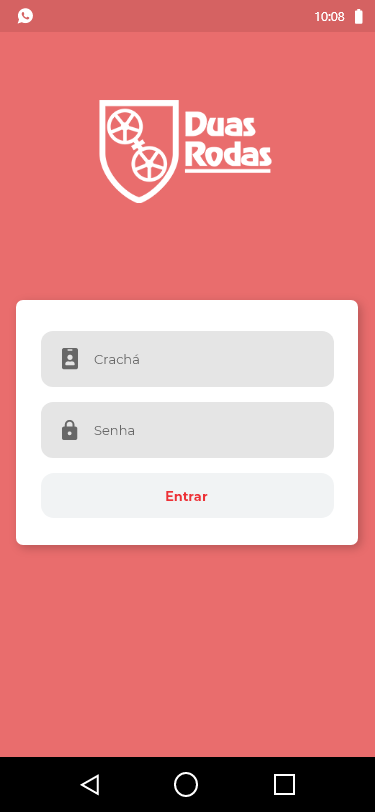
\includegraphics[scale=.65]{Figuras/Login}}\qquad
		
	}	
\end{figure}
\newpage
%--
%Tela de Menu parte superior da tela com informações rápidas sobre ordens de serviços.
Tela de menu foi dividida em duas imagens. Está primeira refere-se a parte superior do menu que contem gráficos para o funcionário acompanhar as ordens em aberto,andamento, e um gráfico maior que pode acompanhar uma visão geral do mês das ordens de serviços.  
\begin{figure}[htb]
	\centering
	\mbox{%
		\subfigure[Tela Menu parte superior da tela]{\label{MENU}%
			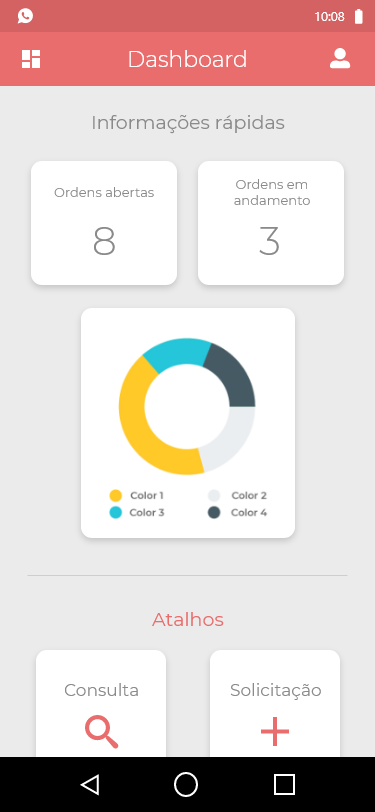
\includegraphics[scale=.65]{Figuras/MENU}}
	}	
	
\end{figure}
% ---
\newpage
%Figura "a", tela principal com finalidade de mostrar todas as opções do usuário.
%Figura "b", tela para cadastramento de ordem de serviços.
%Tela de Menu parte inferior da tela com finalidade de acesso rápido de cada operação disponível.
Tela de menu segunda imagem, que corresponde aos atalhos para um rápido acesso aos recursos disponíveis do sistema para o funcionário
como consultar ordens de serviço, cadastrar causa,sintoma ou defeito,
solicitar peça para o estoque entre outros recursos.
%\ref{dashboard}
\begin{figure}[htb]
	\centering
	\mbox{%
		\subfigure[Tela Menu parte inferior da tela]{\label{MENU_1}%
			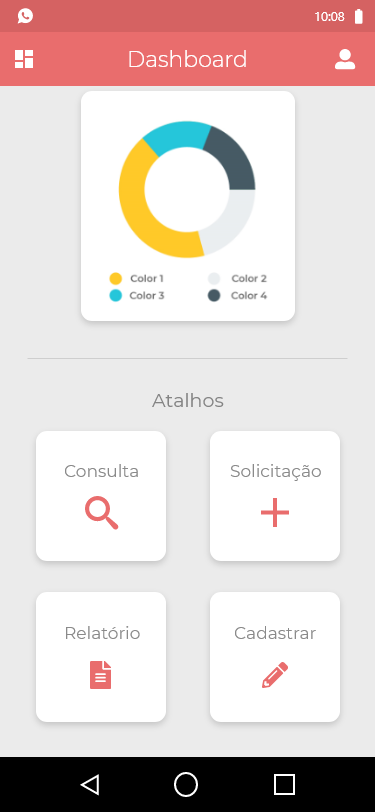
\includegraphics[scale=.65]{Figuras/MENU_1}}
	}	
	
\end{figure}
%--
\newpage
Tela de para cadastrar causa dos problemas da OS e de seus sintomas.
\begin{figure}[htb]
	\centering
	\mbox{%
		\subfigure[Tela defeito e sintoma]{\label{CADASTROS_1}%
			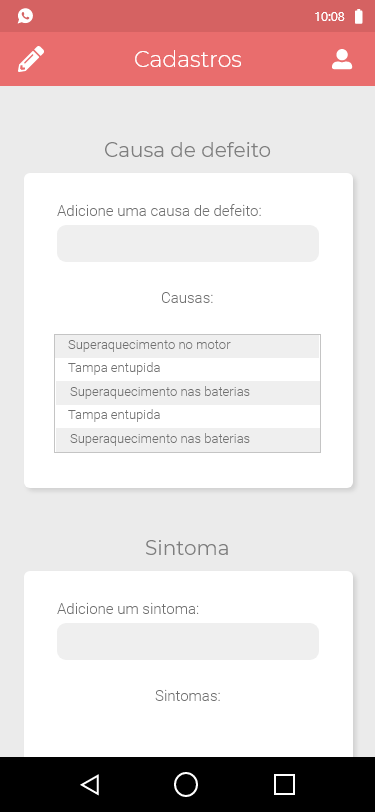
\includegraphics[scale=.65]{Figuras/CADASTROS_1}}\qquad
		
	}
\end{figure}
% ---
\newpage
%Figura "a", telas com finalidades de consultar Ordem Serviço.
%Figura "b", tela para ver os detalhes de cada Ordem de Serviço.
Tela de com opções de detalhamento de ordem de serviço.
%\ref{consulta}
\begin{figure}[htb]
	\centering
	\mbox{%
		
		\subfigure[Tela de opções de Detalhes]{\label{DETALHES_OS_1}%
			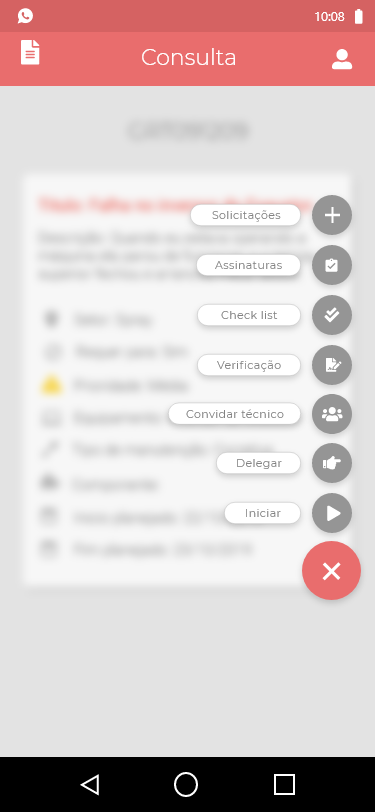
\includegraphics[scale=.65]{Figuras/DETALHES_OS_1}}
	}
	
\end{figure}
\newpage
Tela de cadastro de defeitos apresentados na manutenção também como suas causas de defeito. 
\begin{figure}[htb]
	\centering
	\mbox{%
		\subfigure[Tela de defeito e causa]{\label{CADASTROS}%
			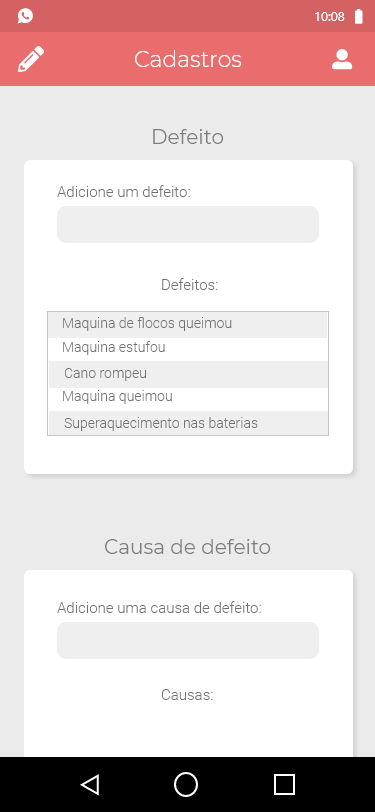
\includegraphics[scale=.65]{Figuras/CADASTROS}}\qquad
		
	}	
\end{figure}
% ---
%\newpage
\newpage
Tela de detalhamento mostrando todos os detalhes da OS.
%Figura "a", telas para verificação de ordem de serviço.
%Figura "b", tela para pegar assinatura dos responsáveis por meio do número do crachás.

%\ref{verificacao}
\begin{figure}[htb]
	\centering
	\mbox{%
		\subfigure[Tela de consulta detalhada]{\label{DETALHES_OS}%
			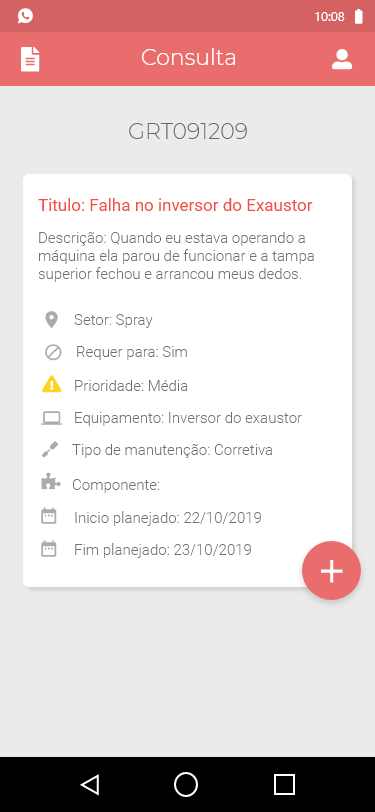
\includegraphics[scale=.65]{Figuras/DETALHES_OS}}\qquad
		
	}	
\end{figure}
\newpage
%--
Tela de consultar de ordens de serviço com filtros por data ,prioridade, status ou suas próprias em minhas os.
\begin{figure}[htb]
	\centering
	\mbox{%
		\subfigure[Tela consultar OS]{\label{CONSULTAR_OS}%
			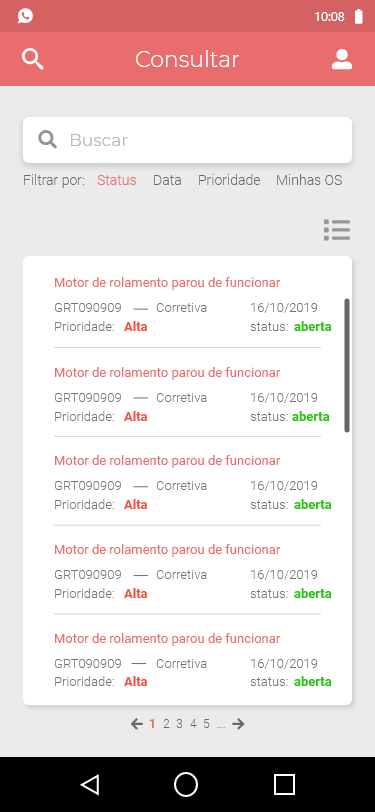
\includegraphics[scale=.65]{Figuras/CONSULTAR_OS}}
	}
\end{figure}
% ---

%Figura "a", telas com finalidade de solicitação de peças.
%Figura "b", tela para realizar apontamento pelo mecânico.
\newpage
Tela para ser solicitada peças para manutenção.

\begin{figure}[htb]
	\centering
	\mbox{%
		\subfigure[Tela Solicitação de Peça]{\label{SOLICITACOES_DE_PECAS}%
			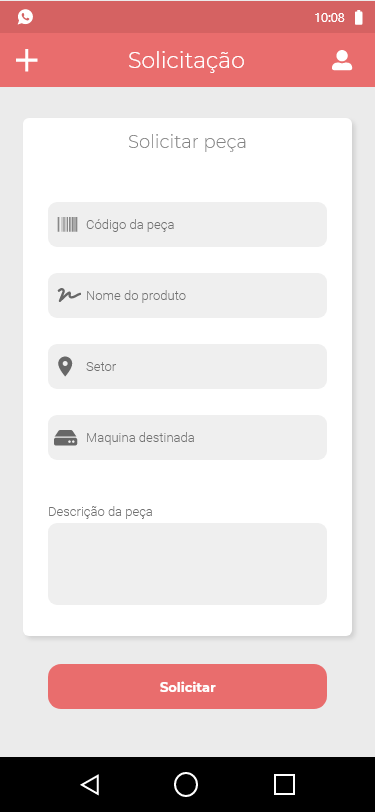
\includegraphics[scale=.65]{Figuras/SOLICITACOES_DE_PECAS}}\qquad
	}
	
\end{figure}
\newpage
Tela de verificação, apontamento e assinatura para realizar o funcionário se o problema foi resolvido, apontar horas trabalhadas e coletar assinatura.
\begin{figure}[htb]
	\centering
	\mbox{%
		
		\subfigure[Tela Verificação]{\label{VERIFICACAO}%
			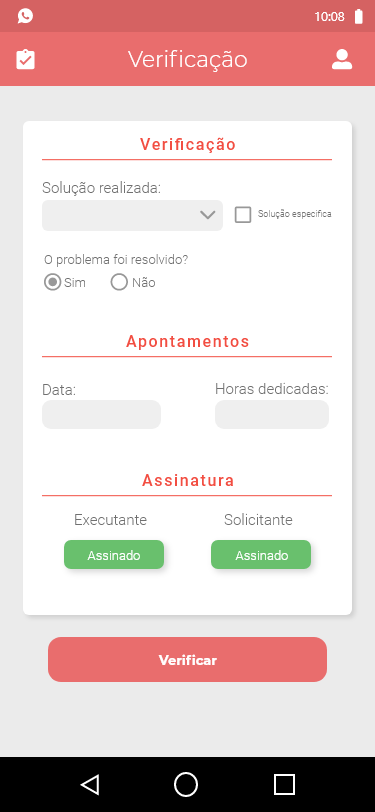
\includegraphics[scale=.65]{Figuras/VERIFICACAO}}
	}	
	
\end{figure}
\newpage

Tela de verificação mostrando o processo de assinatura do executante e do seu solicitante.

\begin{figure}[htb]
	\centering
	\mbox{%
		\subfigure[Tela Verificação Assinatura]{\label{VERIFICACAO_2}%
			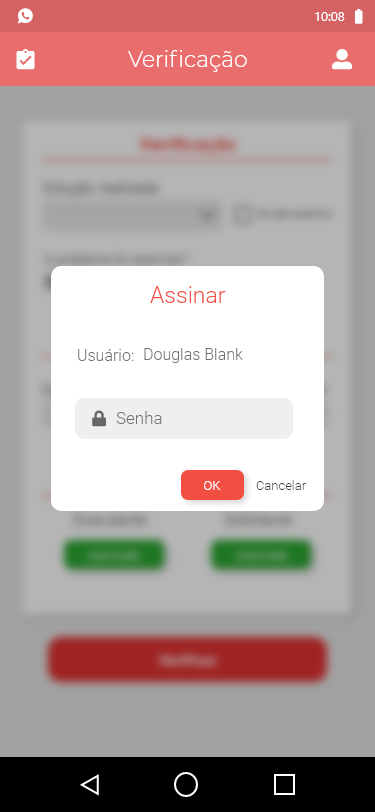
\includegraphics[scale=.65]{Figuras/VERIFICACAO_2.png}}\qquad
	}	
	
\end{figure}
\newpage
Tela das assinaturas para verificar se o processo teve a aprovação dos responsáveis em cada etapa realizada.

\begin{figure}[htb]
	\centering
	\mbox{%
		\subfigure[Tela Apontado]{\label{ASSINATURAS}%
			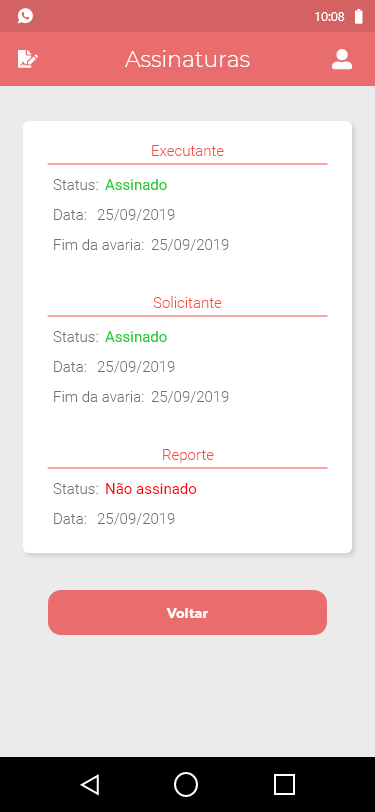
\includegraphics[scale=.65]{Figuras/ASSINATURAS}}
	}
	
\end{figure}

\newpage

Tela de Checklist dos equipamentos de proteção individual.
\begin{figure}[htb]
	\centering
	\mbox{%
		\subfigure[Tela EPI]{\label{EPI}%
			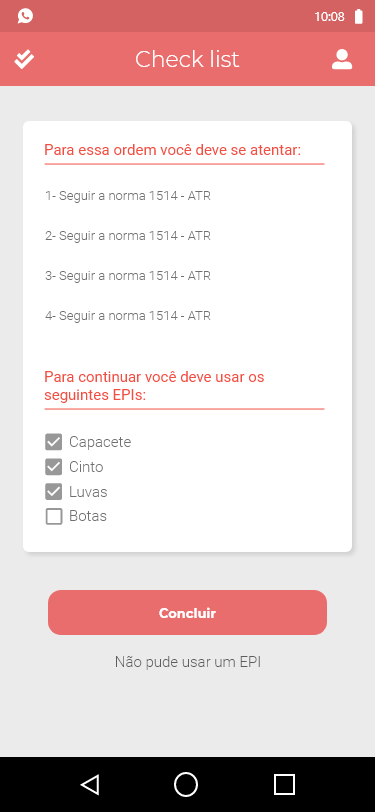
\includegraphics[scale=.65]{Figuras/EPI}}
	}
	
\end{figure}

\newpage

Tela para se justificação do motivo por não utilizar algum EPI especifico.

\begin{figure}[htb]
	\centering
	\mbox{%
		\subfigure[Tela justificação não uso EPI]{\label{EPI_1}%
			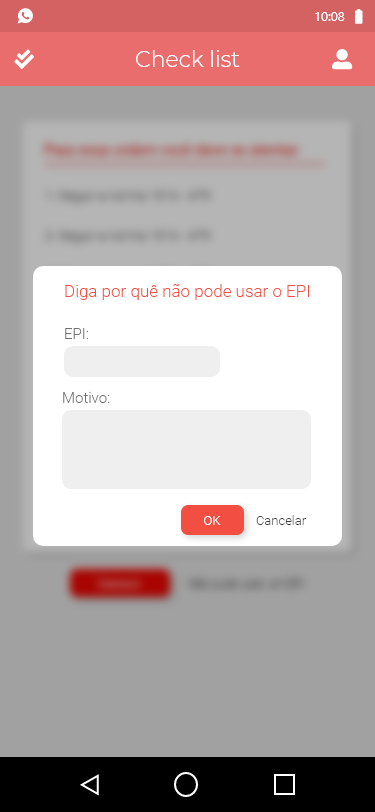
\includegraphics[scale=.65]{Figuras/EPI_1}}\qquad
	}
	
\end{figure}
\newpage
% ---
% ---

\begin{center}
	Protótipos da parte WEB.
\end{center}


Tela para se realizar o login no sistema WEB.

\begin{figure}[H]
	\centering
	\mbox{%
		\subfigure[Tela de login]{\label{LOGIN_1}%
			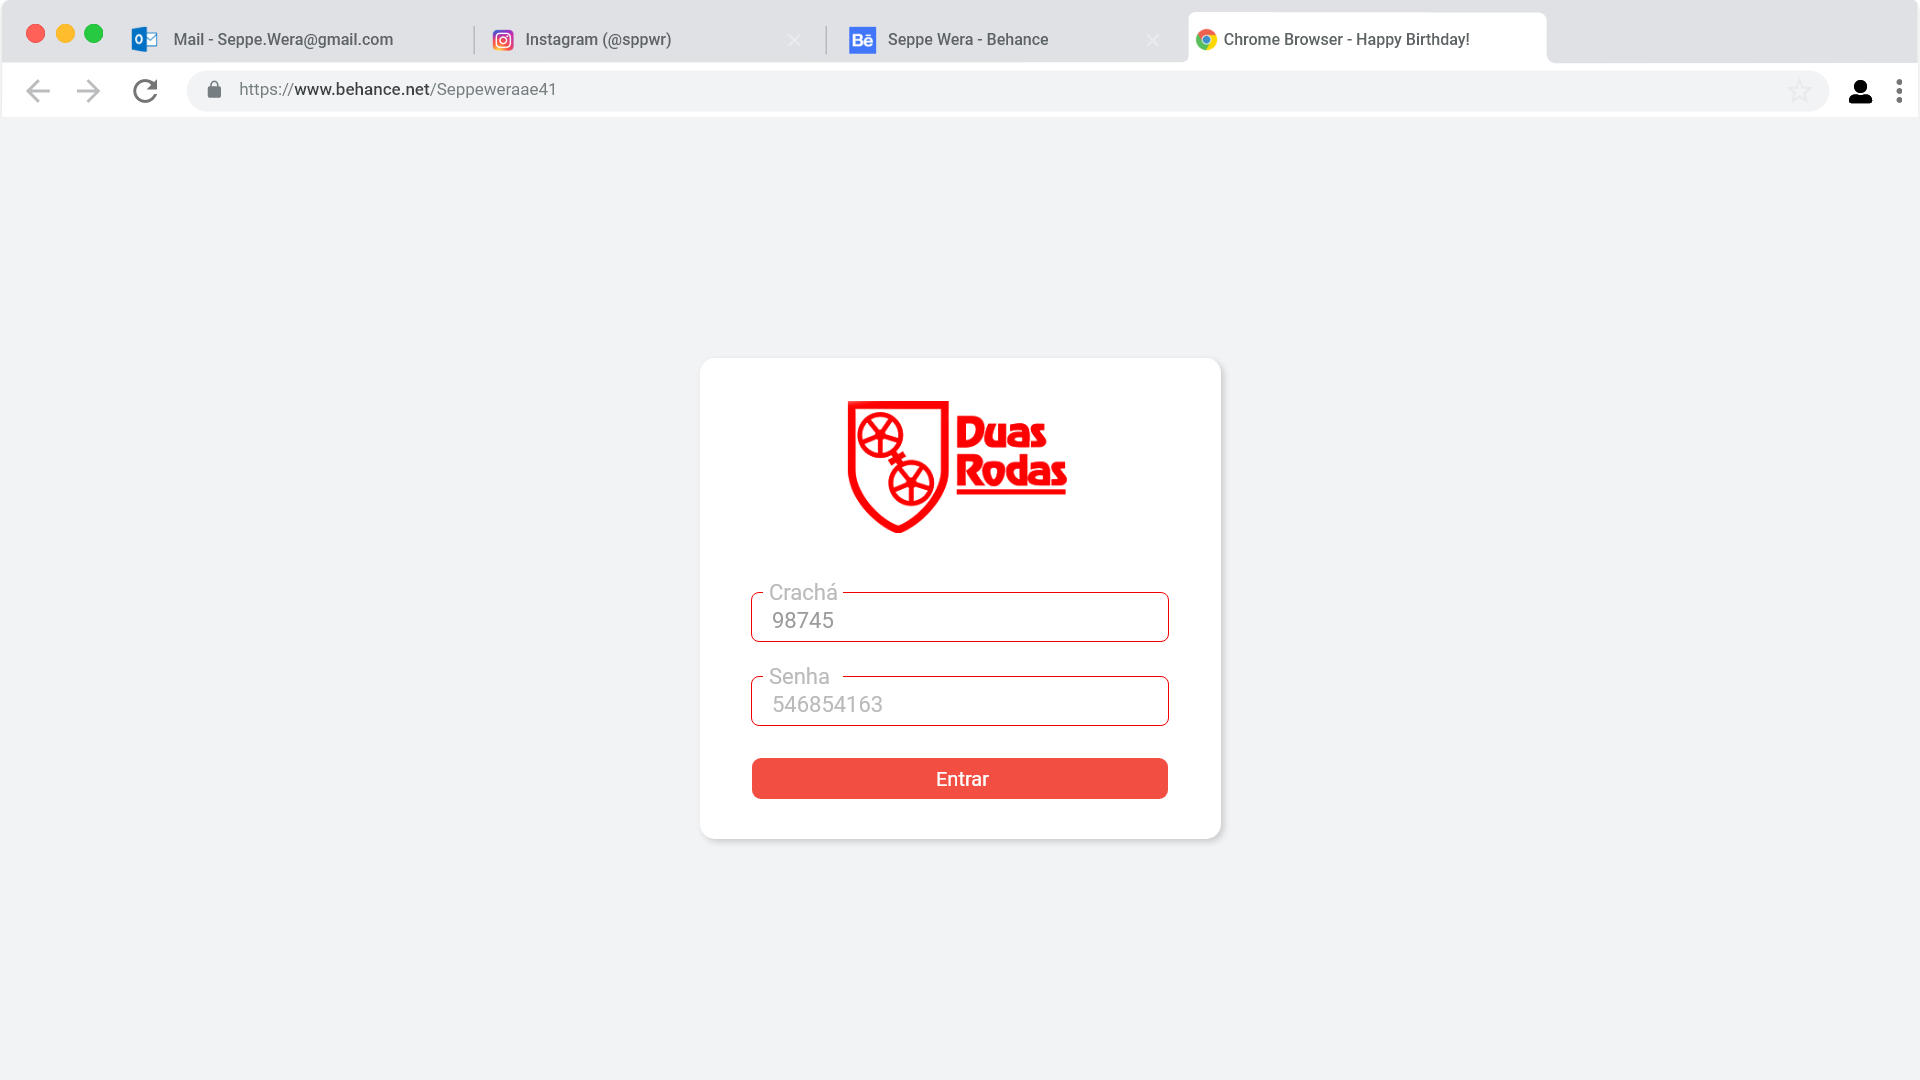
\includegraphics[scale=.32,angle=90]{Figuras/LOGIN_1}}\qquad
	}
	
\end{figure}
\newpage
Tela de dashboard com as peçotes disponíveis no sistema assim como gráficos e relatórios das OS.

\begin{figure}[htb]
	\centering
	\mbox{%
		\subfigure[Tela de dashboard]{\label{DASHBOARD_2}%
			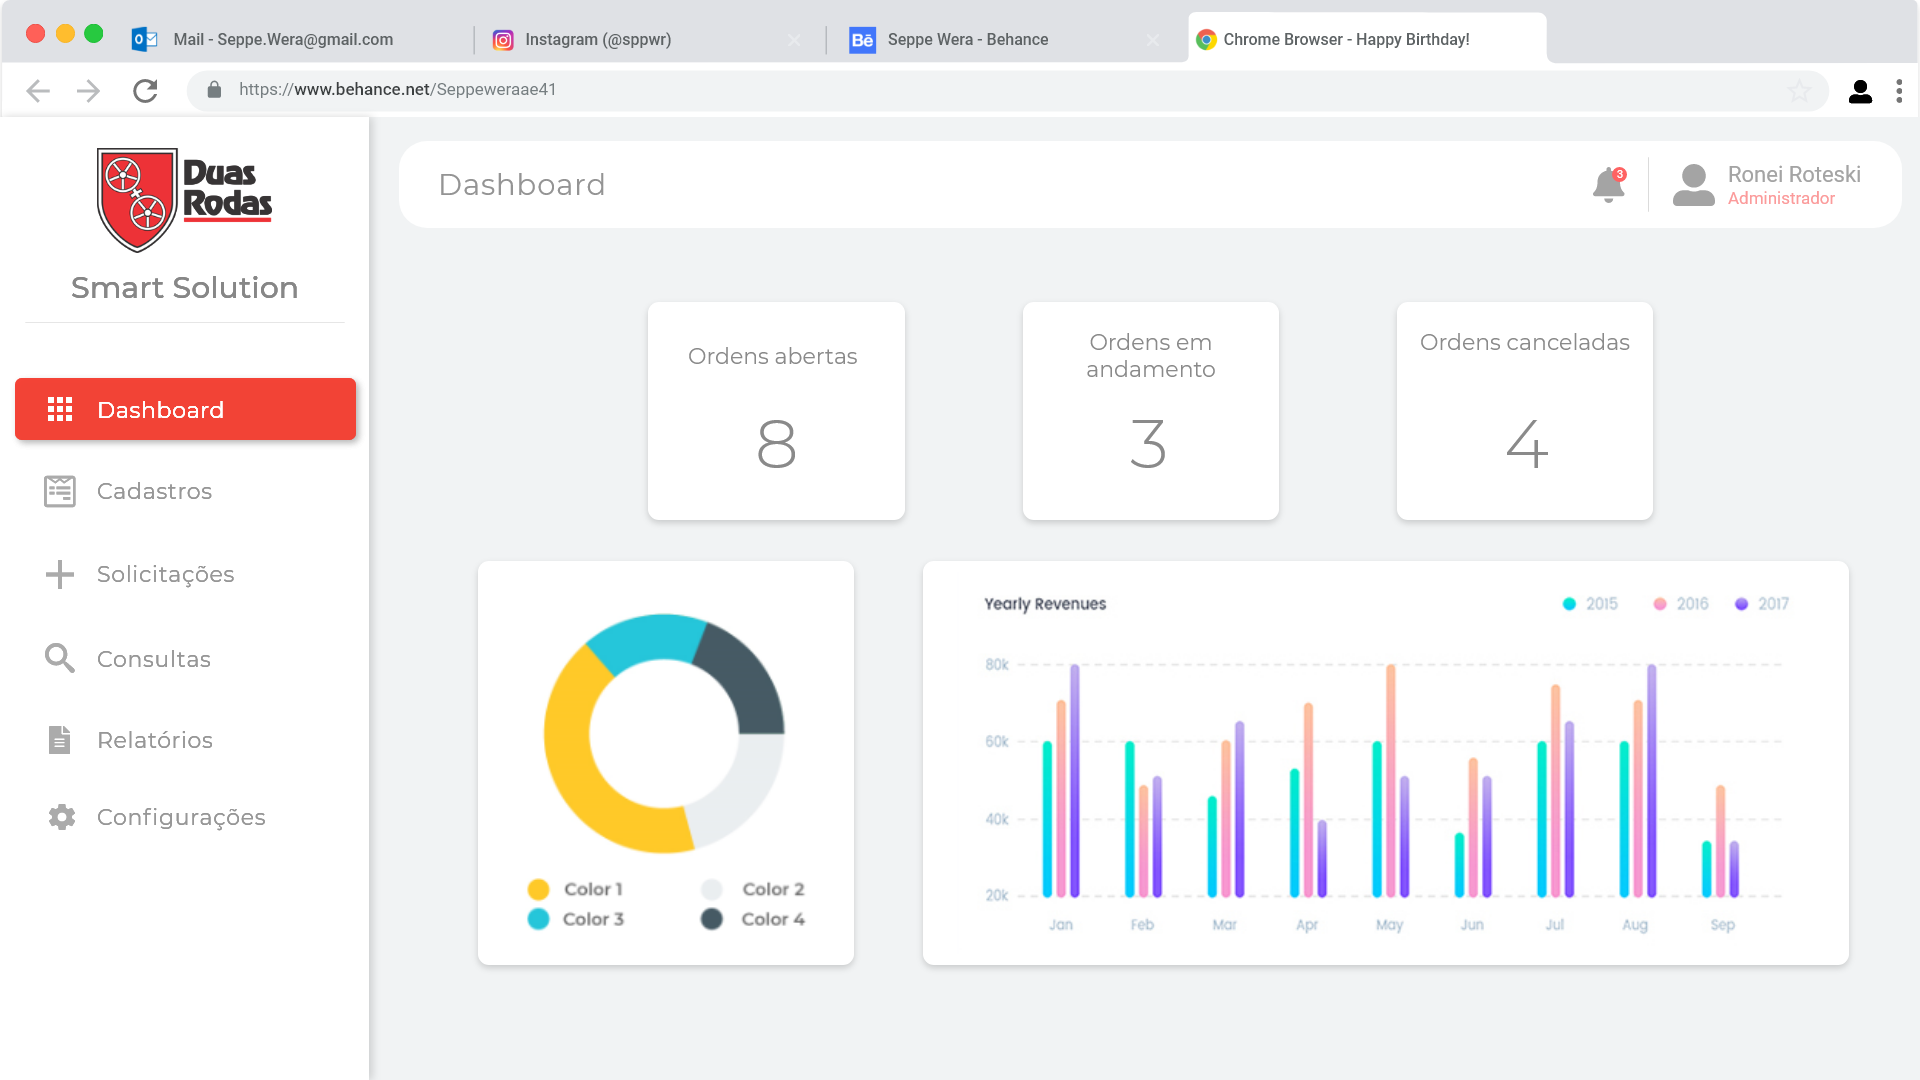
\includegraphics[scale=.32,angle=90]{Figuras/DASHBOARD_2}}\qquad
	}
	
\end{figure}
\newpage

Tela com as opções de cadastramentos disponíveis no sistema.

\begin{figure}[htb]
	\centering
	\mbox{%
		\subfigure[Tela de Cadastramento]{\label{CADASTROS_3}%
			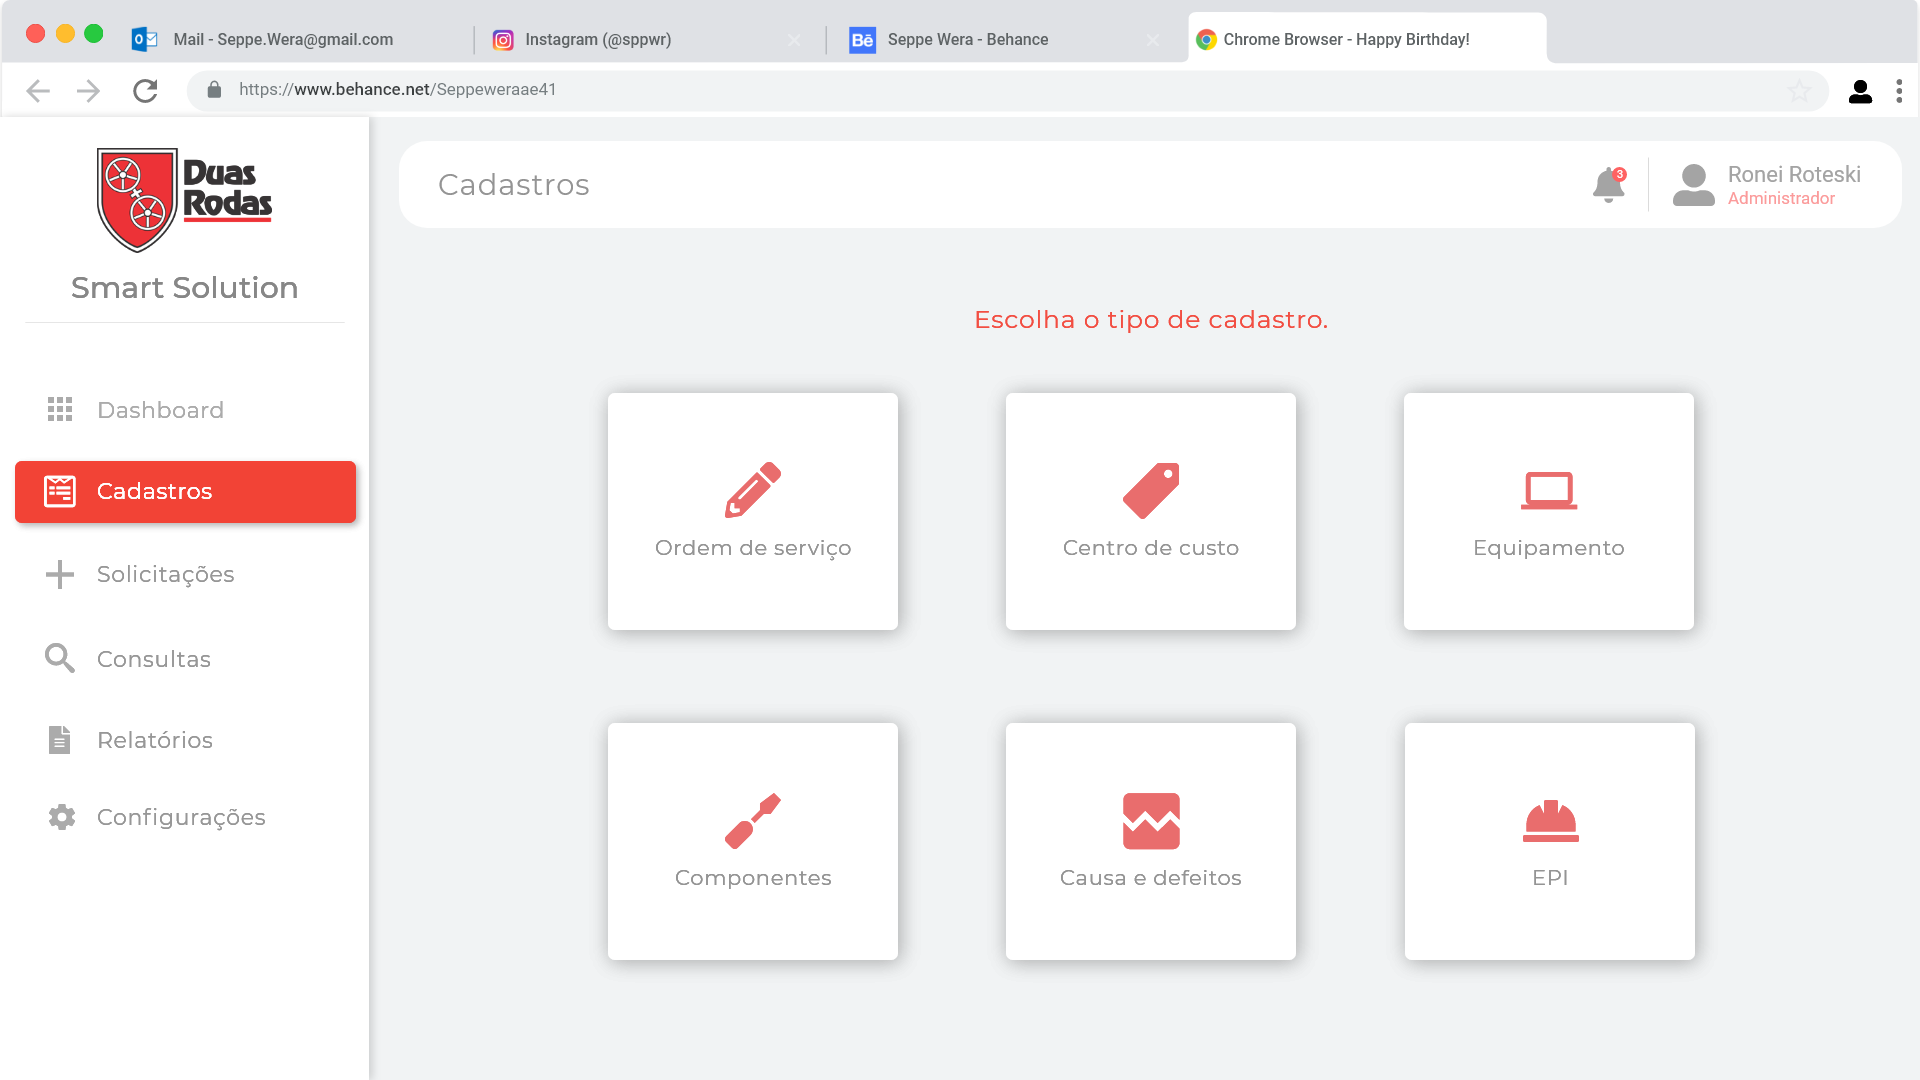
\includegraphics[scale=.32,angle=90]{Figuras/CADASTROS_3}}\qquad
	}
	
\end{figure}
\newpage
Tela para se cadastrar ordem de serviços no sistema de forma manual.

\begin{figure}[htb]
	\centering
	\mbox{%
		\subfigure[Tela cadastro OS]{\label{CADASTRO_OS_4}%
			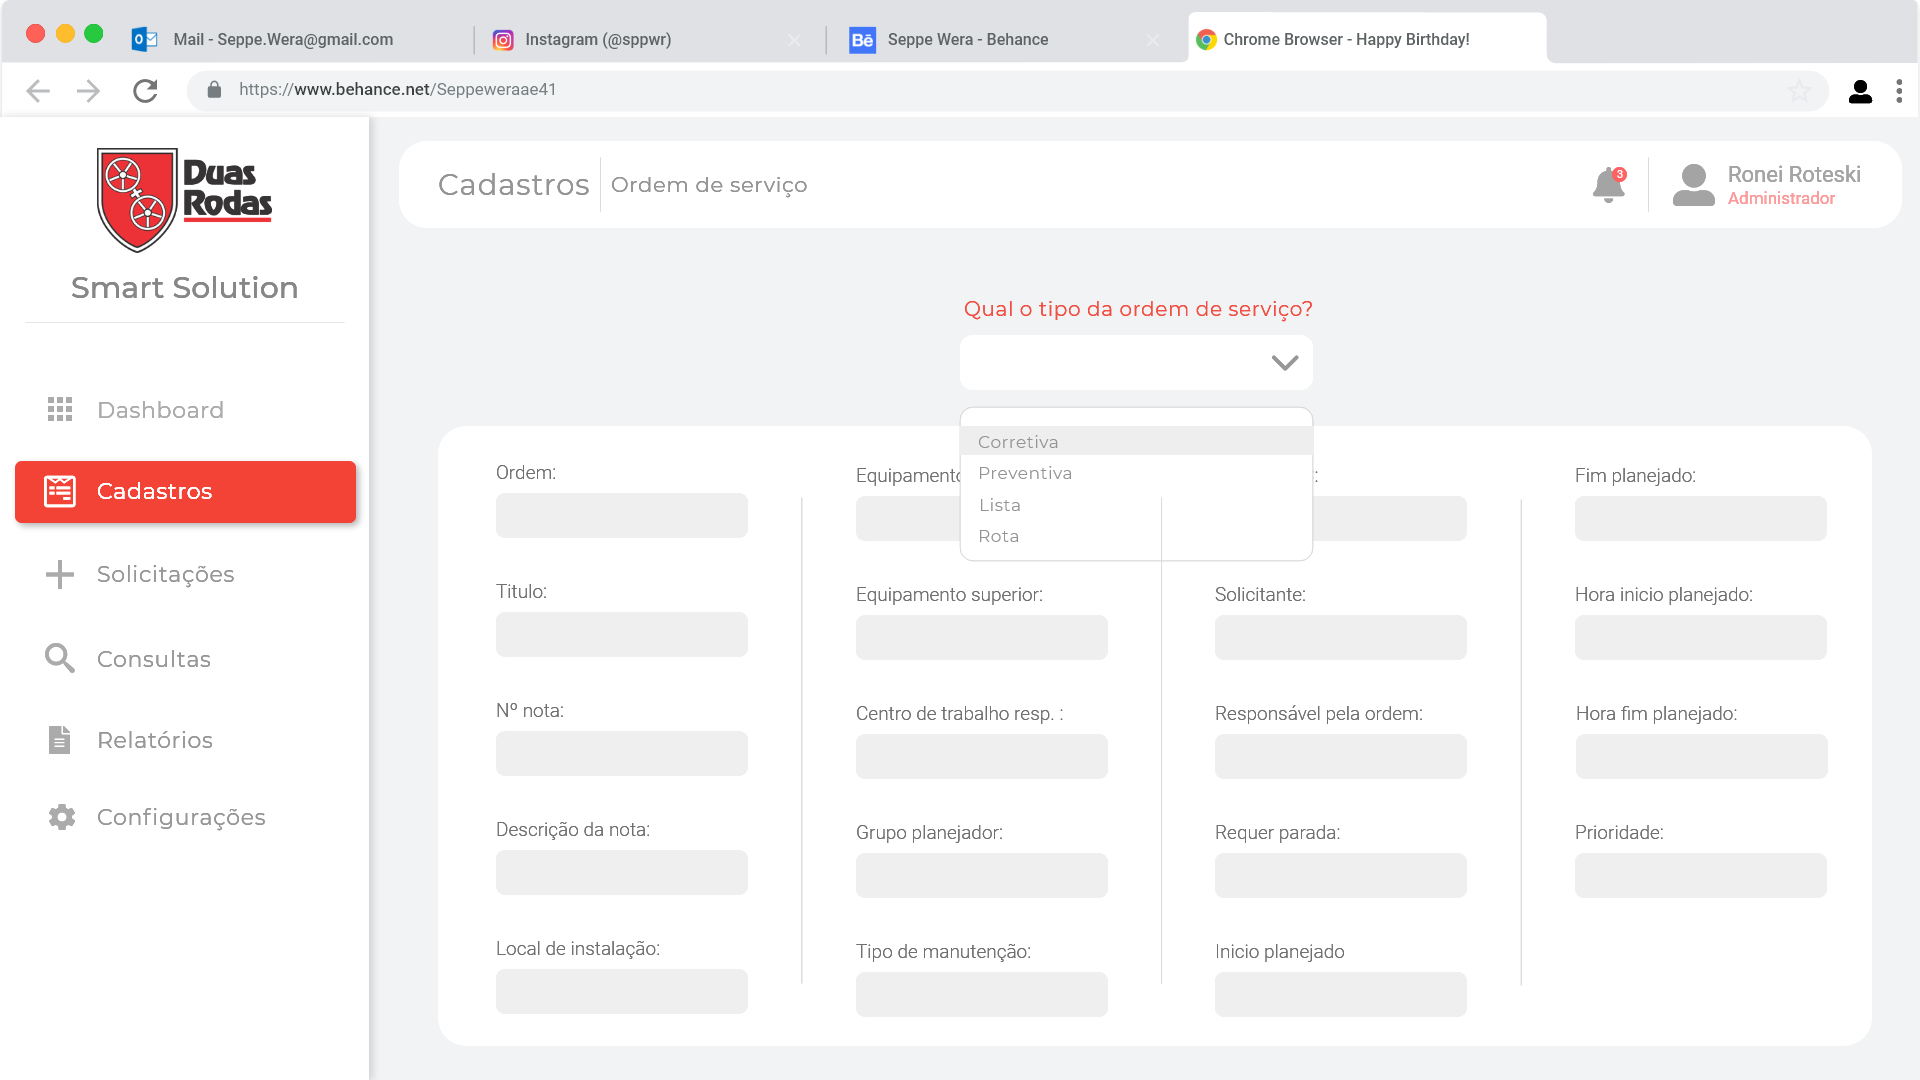
\includegraphics[scale=.32,angle=90]{Figuras/CADASTRO_OS_4}}\qquad
	}
	
\end{figure}
\newpage

Tela para cadastrar equipamentos no sistema.

\begin{figure}[htb]
	\centering
	\mbox{%
		\subfigure[Tela cadastro equipamento]{\label{CADASTRO_EQUIPAMENTO_5}%
			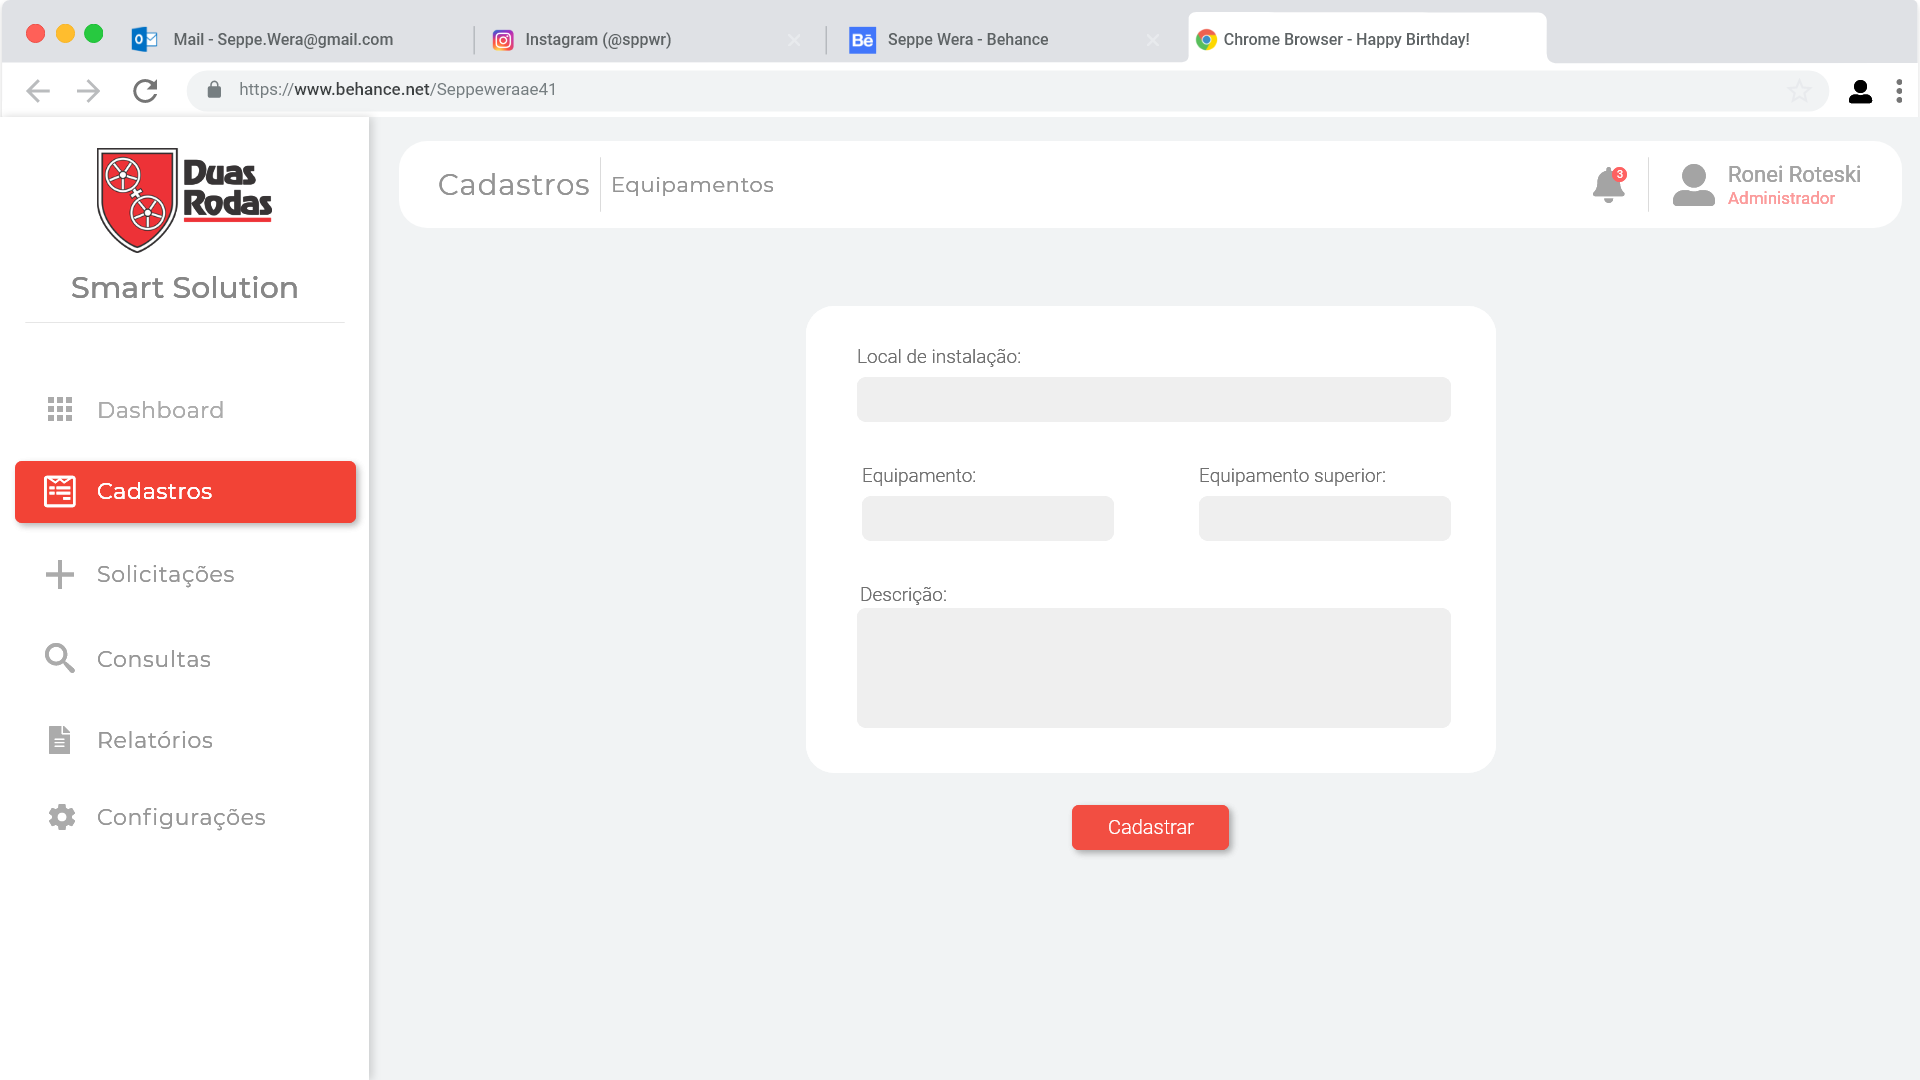
\includegraphics[scale=.32,angle=90]{Figuras/CADASTRO_EQUIPAMENTO_5}}\qquad
	}
	
\end{figure}
\newpage

Tela para cadastrar componentes de cada maquina.

\begin{figure}[htb]
	\centering
	\mbox{%
		\subfigure[Tela de cadastros de componentes]{\label{CADASTRO_COMPONENTE_6}%
			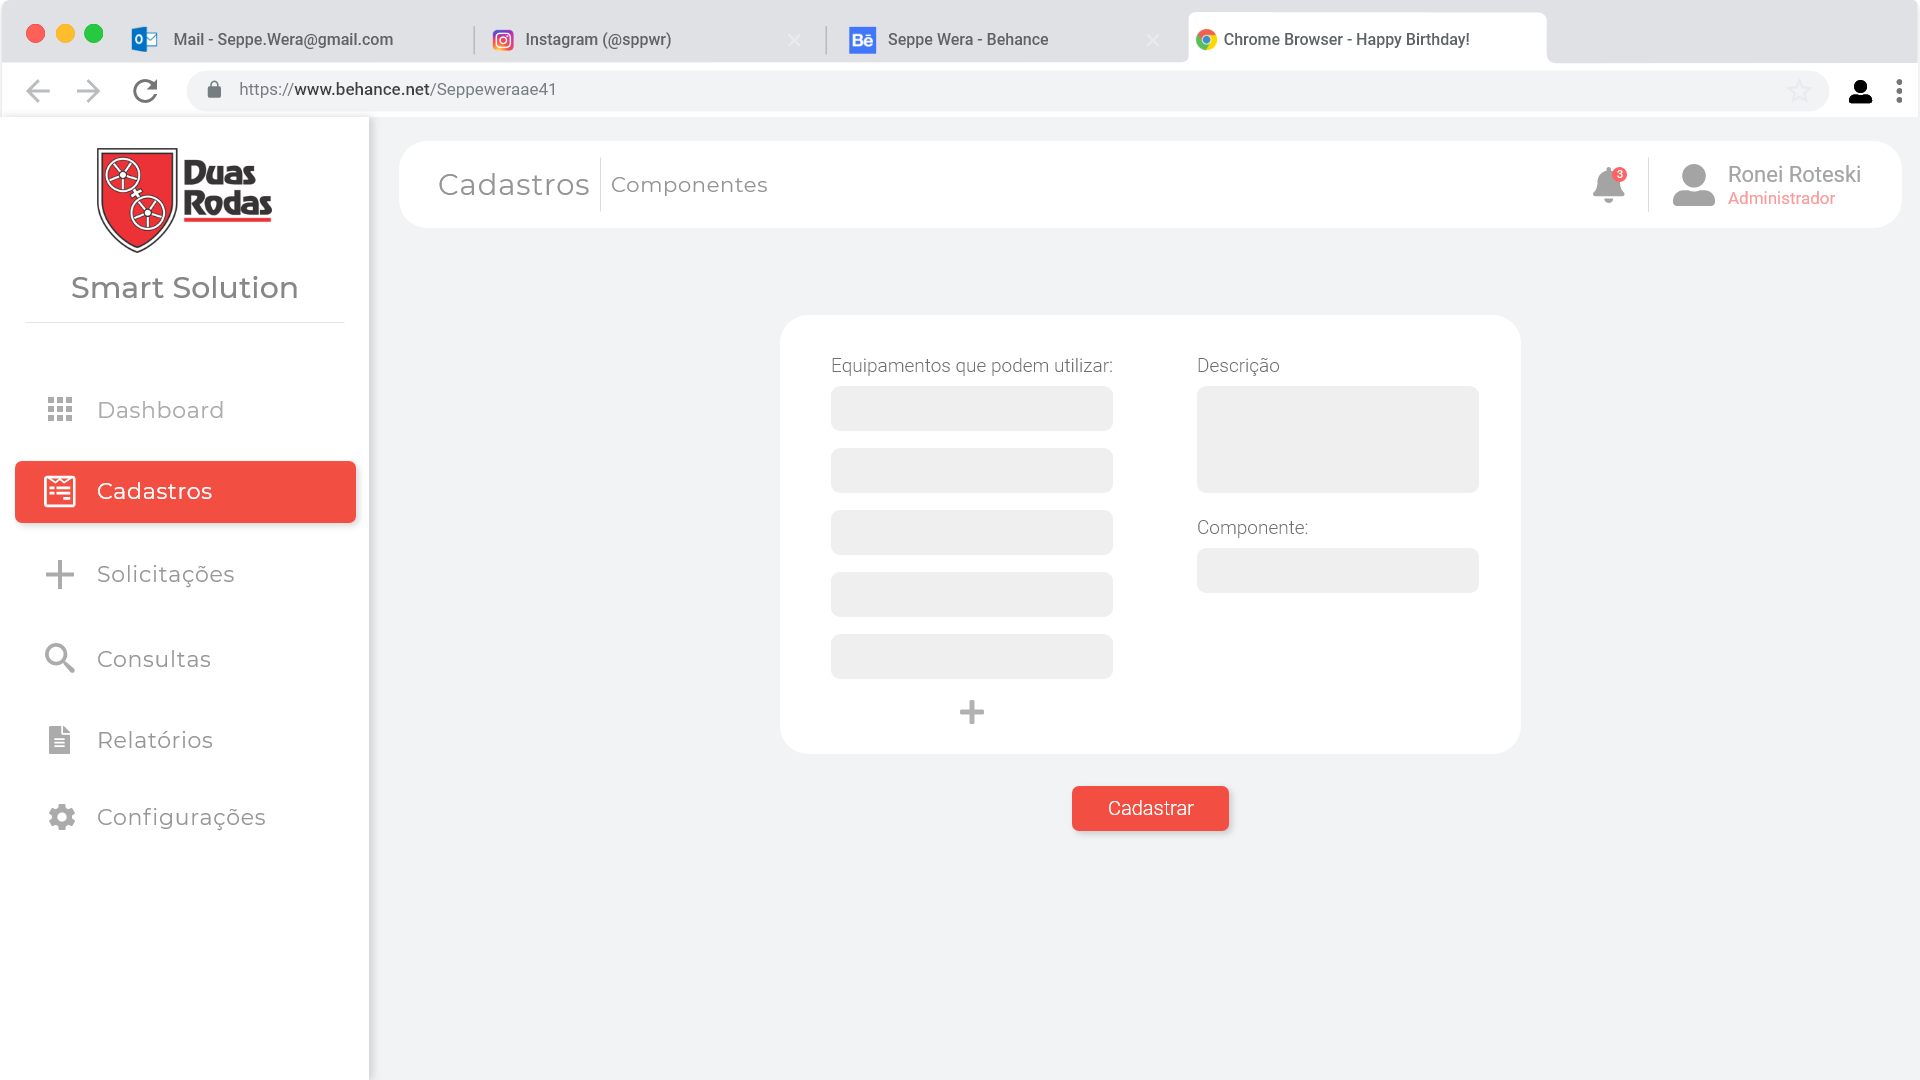
\includegraphics[scale=.32,angle=90]{Figuras/CADASTRO_COMPONENTE_6}}\qquad
	}
	
\end{figure}

\newpage

Tela com finalidade de cadastrar EPI.

\begin{figure}[htb]
	\centering
	\mbox{%
		\subfigure[Tela cadastro EPI]{\label{CADASTRO_EPI_7}%
			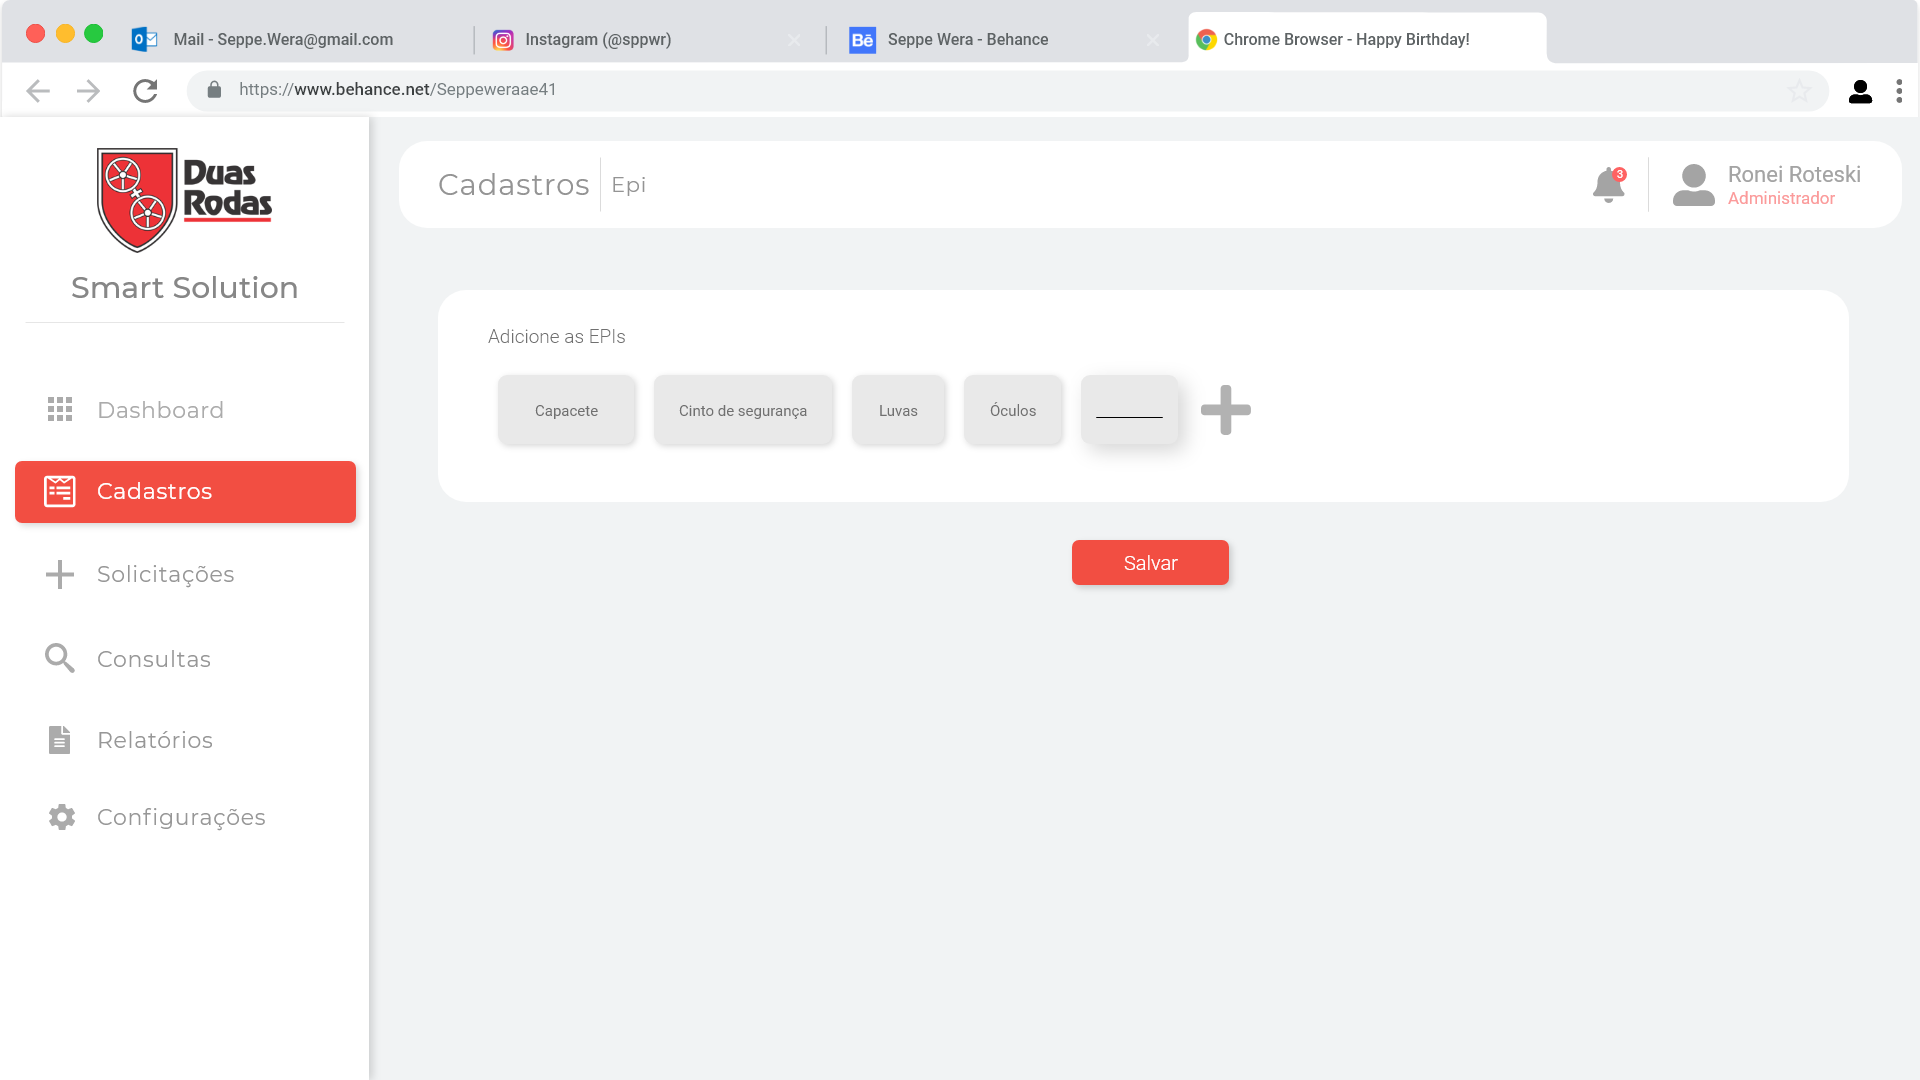
\includegraphics[scale=.32,angle=90]{Figuras/CADASTRO_EPI_7}}\qquad
	}
	
\end{figure}
\newpage
Tela para cadastrar causas e sintomas que ja ocorrerão ou novos.

\begin{figure}[htb]
	\centering
	\mbox{%
		\subfigure[Tela cadastro causas e sintomas]{\label{CADASTRO_causa_8}%
			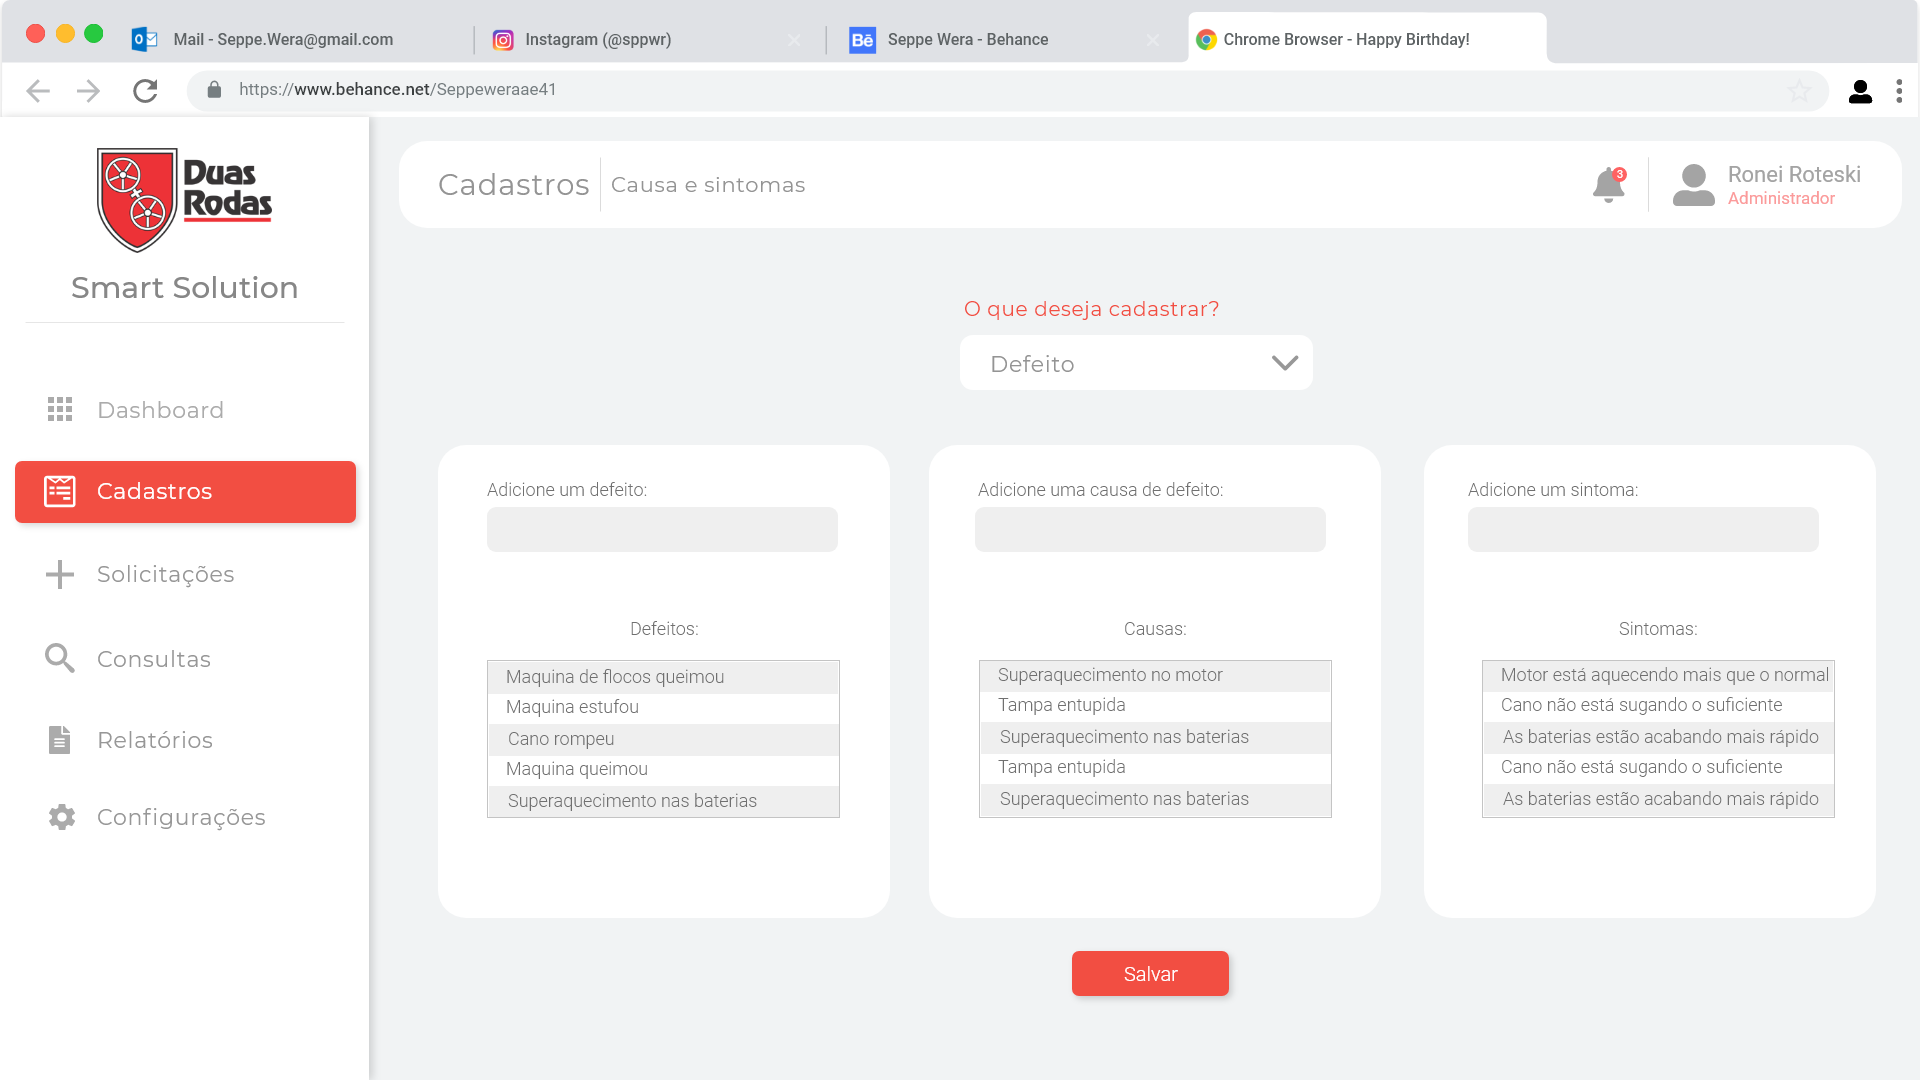
\includegraphics[scale=.32,angle=90]{Figuras/CADASTRO_causa_8}}\qquad
	}
	
\end{figure}
\newpage
Tela para cadastrar operações realizadas com lista disponível para evitar duplicar o mesmo procedimentos.

\begin{figure}[htb]
	\centering
	\mbox{%
		\subfigure[Tela cadastro de operações]{\label{CADASTRO_DE_OPERACOES_9}%
			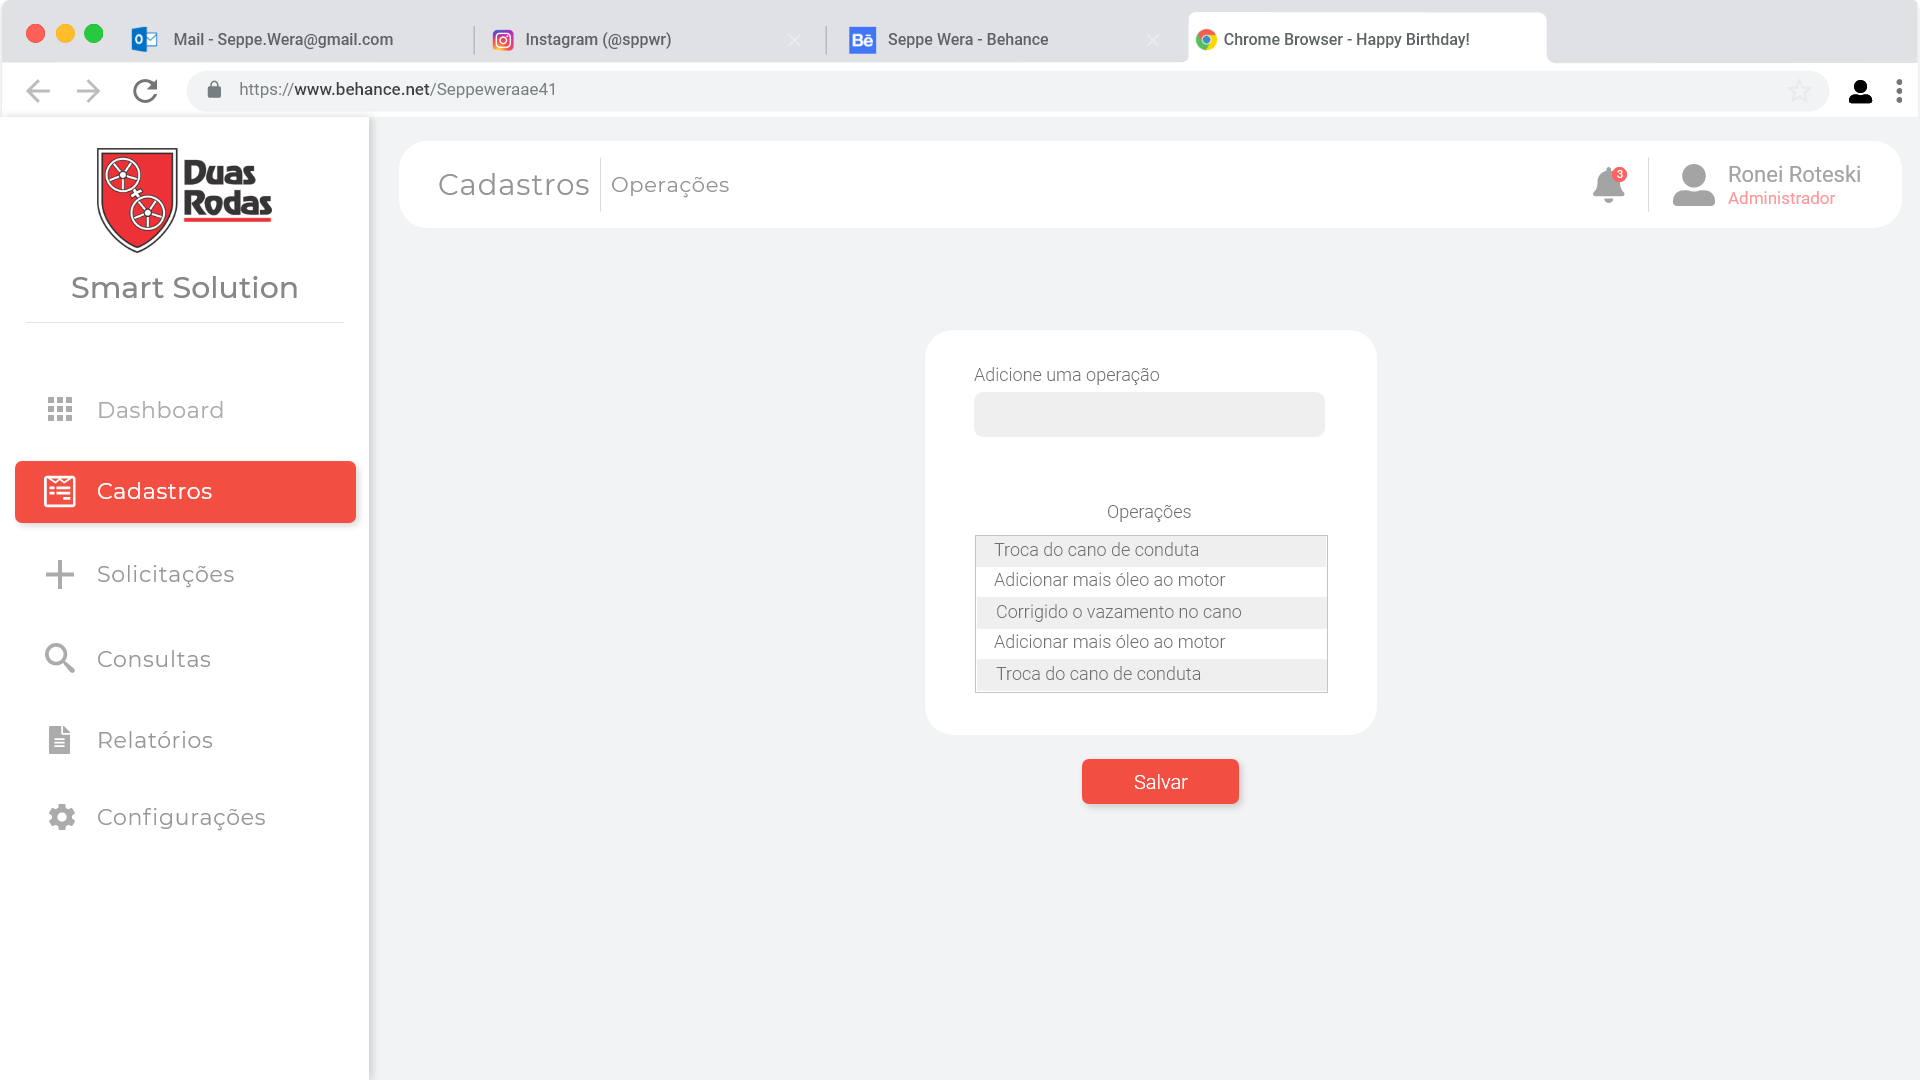
\includegraphics[scale=.32,angle=90]{Figuras/CADASTRO_DE_OPERACOES_9}}\qquad
	}
	
\end{figure}
\newpage
Tela para para se solicitar peças para OS previamente ou apos iniciar-se a ordem de serviço. 

\begin{figure}[htb]
	\centering
	\mbox{%
		\subfigure[Tela para solicitar peças]{\label{Solicitacao_10}%
			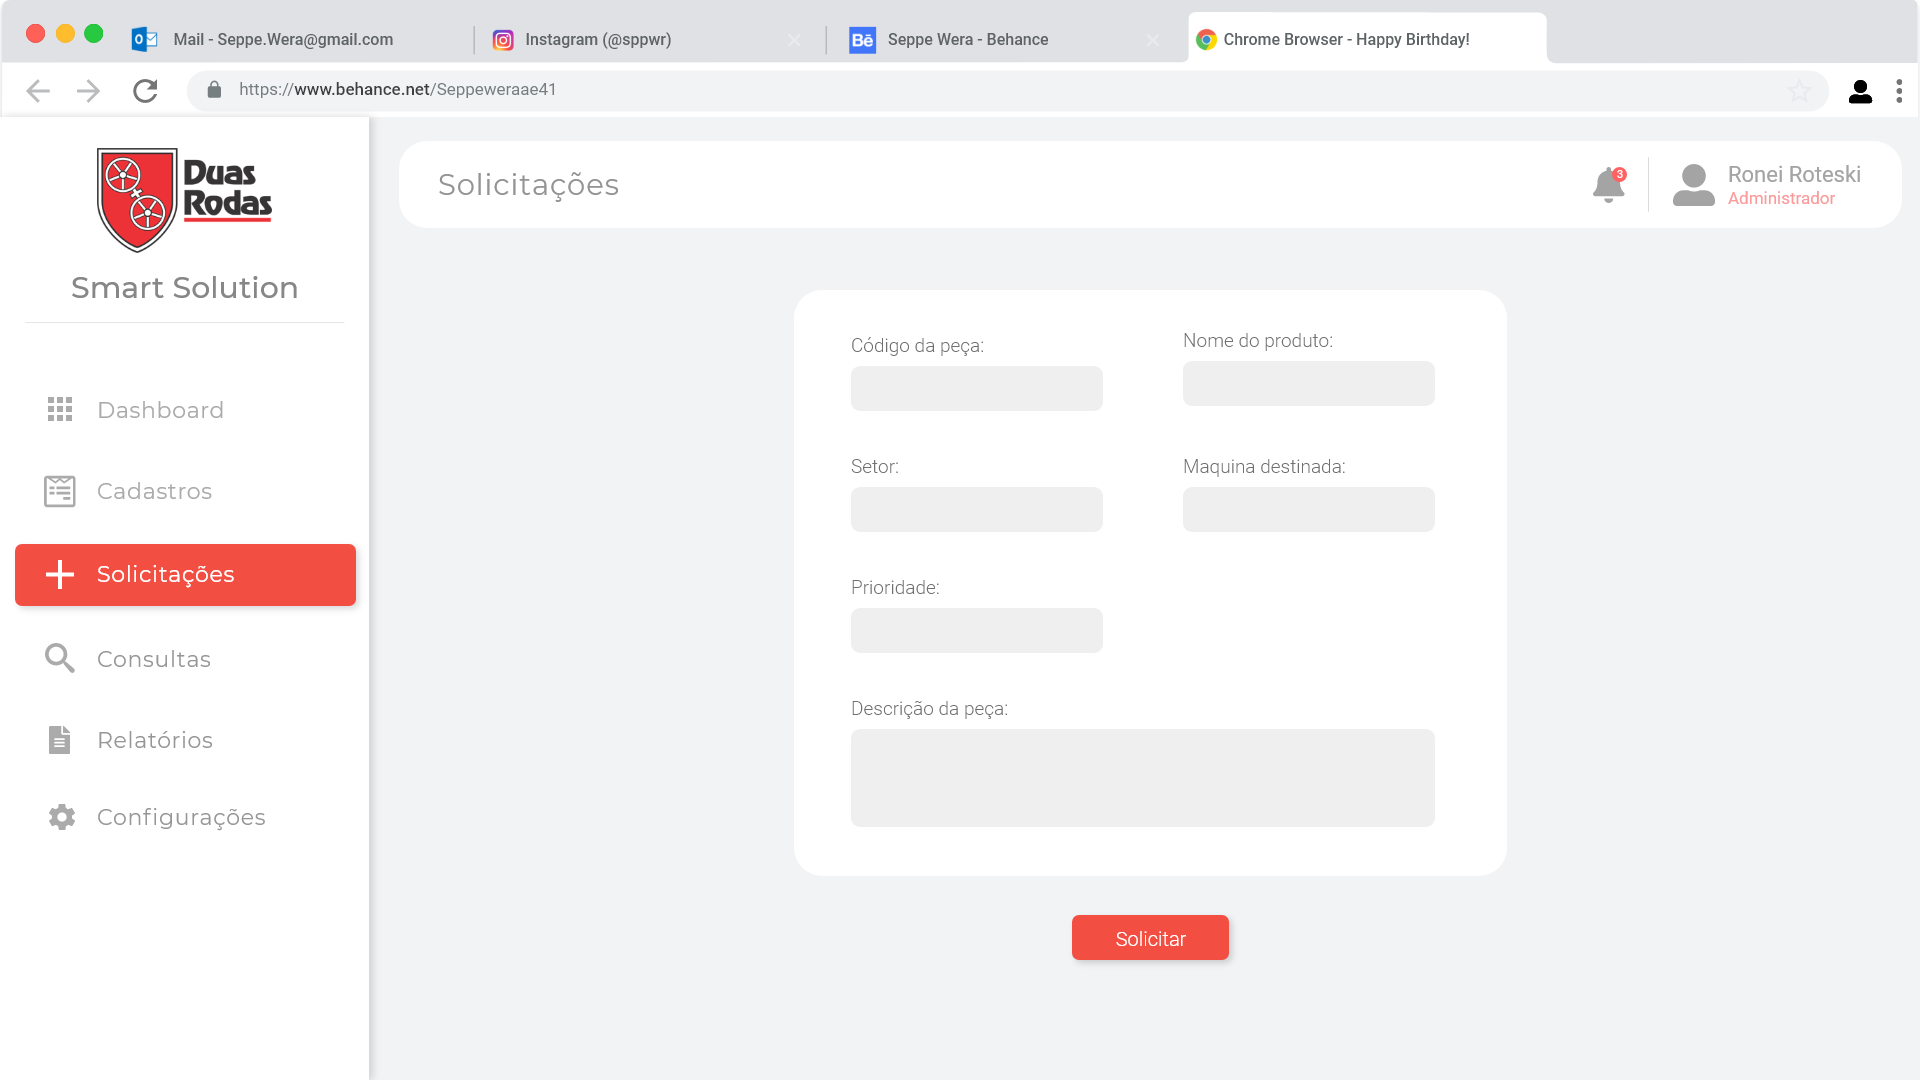
\includegraphics[scale=.32,angle=90]{Figuras/Solicitacao_10}}\qquad
	}
	
\end{figure}
\newpage
Tela de consultar de ordens de serviço com filtros por data ,prioridade, status ou suas próprias em minhas os na parte web.

\begin{figure}[htb]
	\centering
	\mbox{%
		\subfigure[Tela consulta OS]{\label{CONSULTA_11}%
			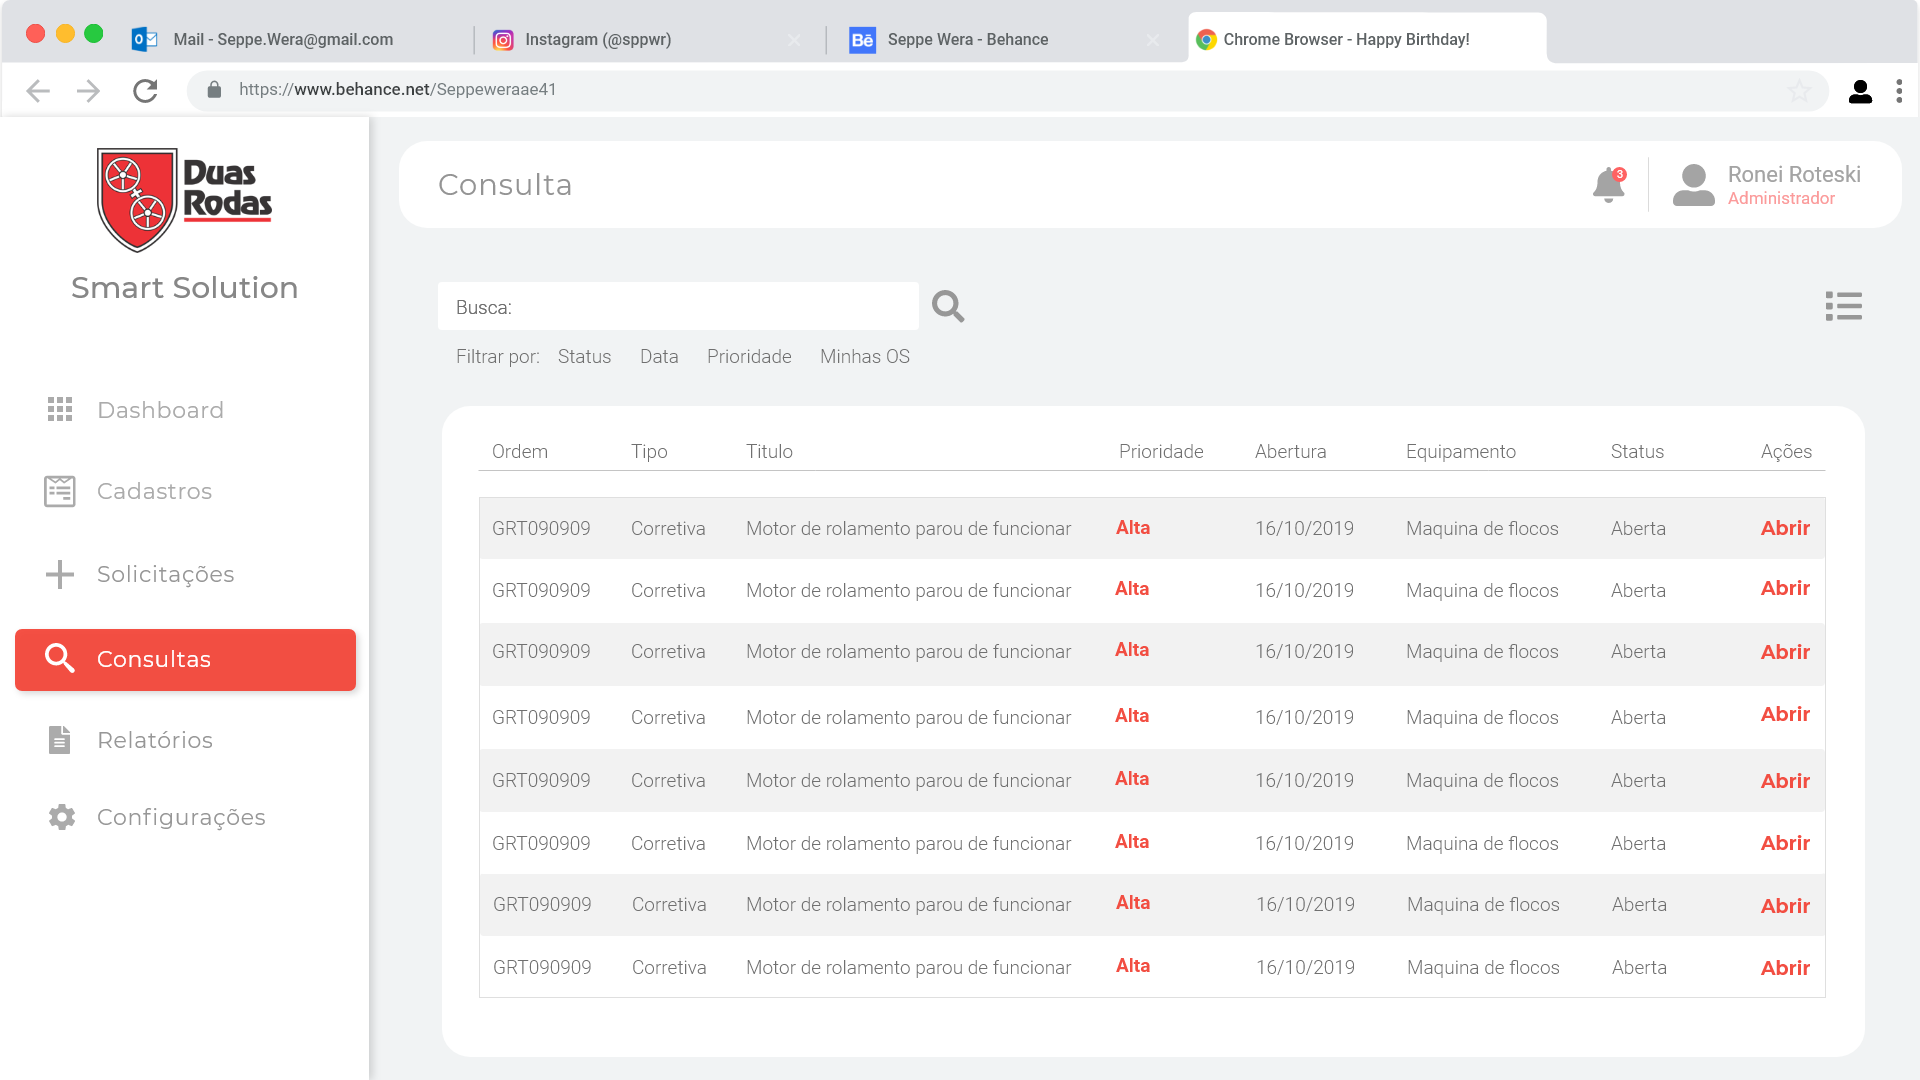
\includegraphics[scale=.32,angle=90]{Figuras/CONSULTA_11}}\qquad
	}
	
\end{figure}
\newpage
Tela de detalhamento de ordem de serviço, com todos as informações da OS e suas opções disponíveis.

\begin{figure}[htb]
	\centering
	\mbox{%
		\subfigure[Tela detalhamento OS]{\label{DETALHAMENTO_12}%
			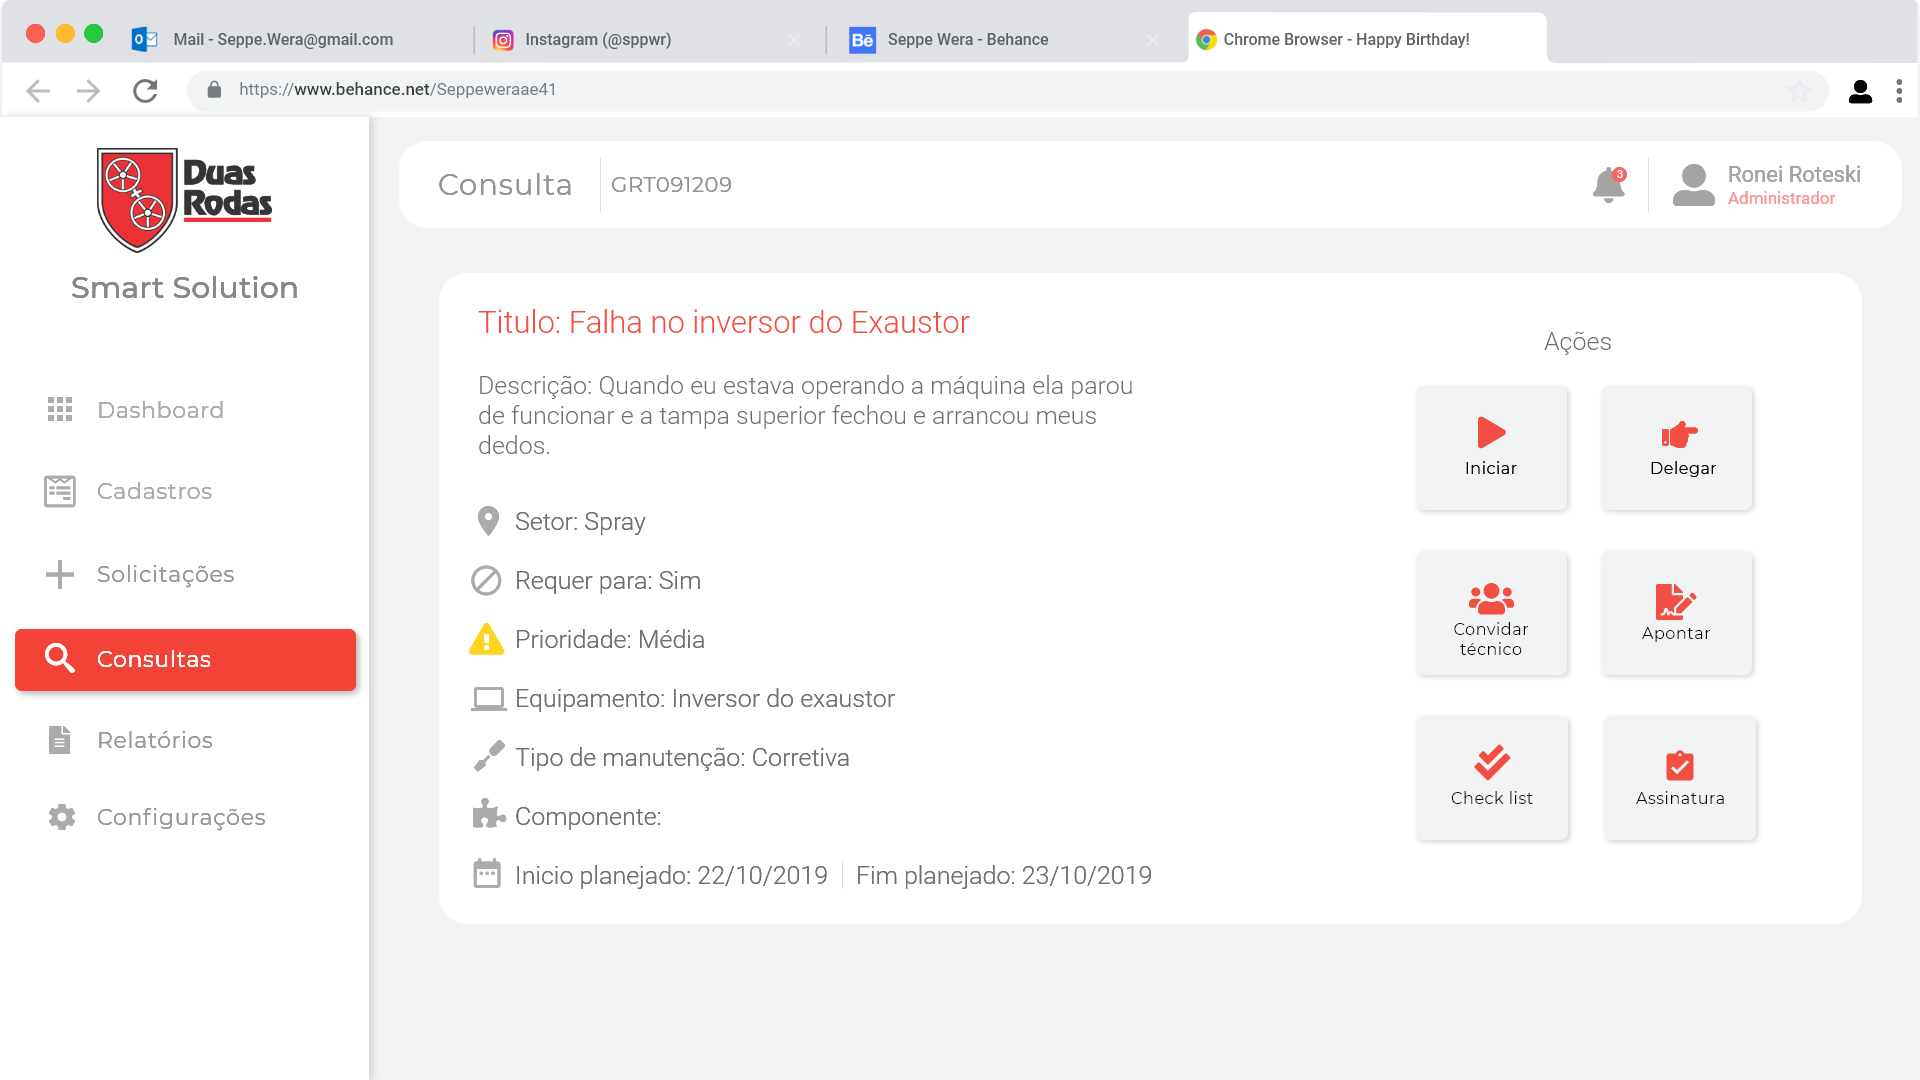
\includegraphics[scale=.32,angle=90]{Figuras/DETALHAMENTO_12}}\qquad
	}
	
\end{figure}
\newpage
Tela de verificação, se o conserto foi concluído.

\begin{figure}[htb]
	\centering
	\mbox{%
		\subfigure[Tela de verificação]{\label{Verificacao_web}%
			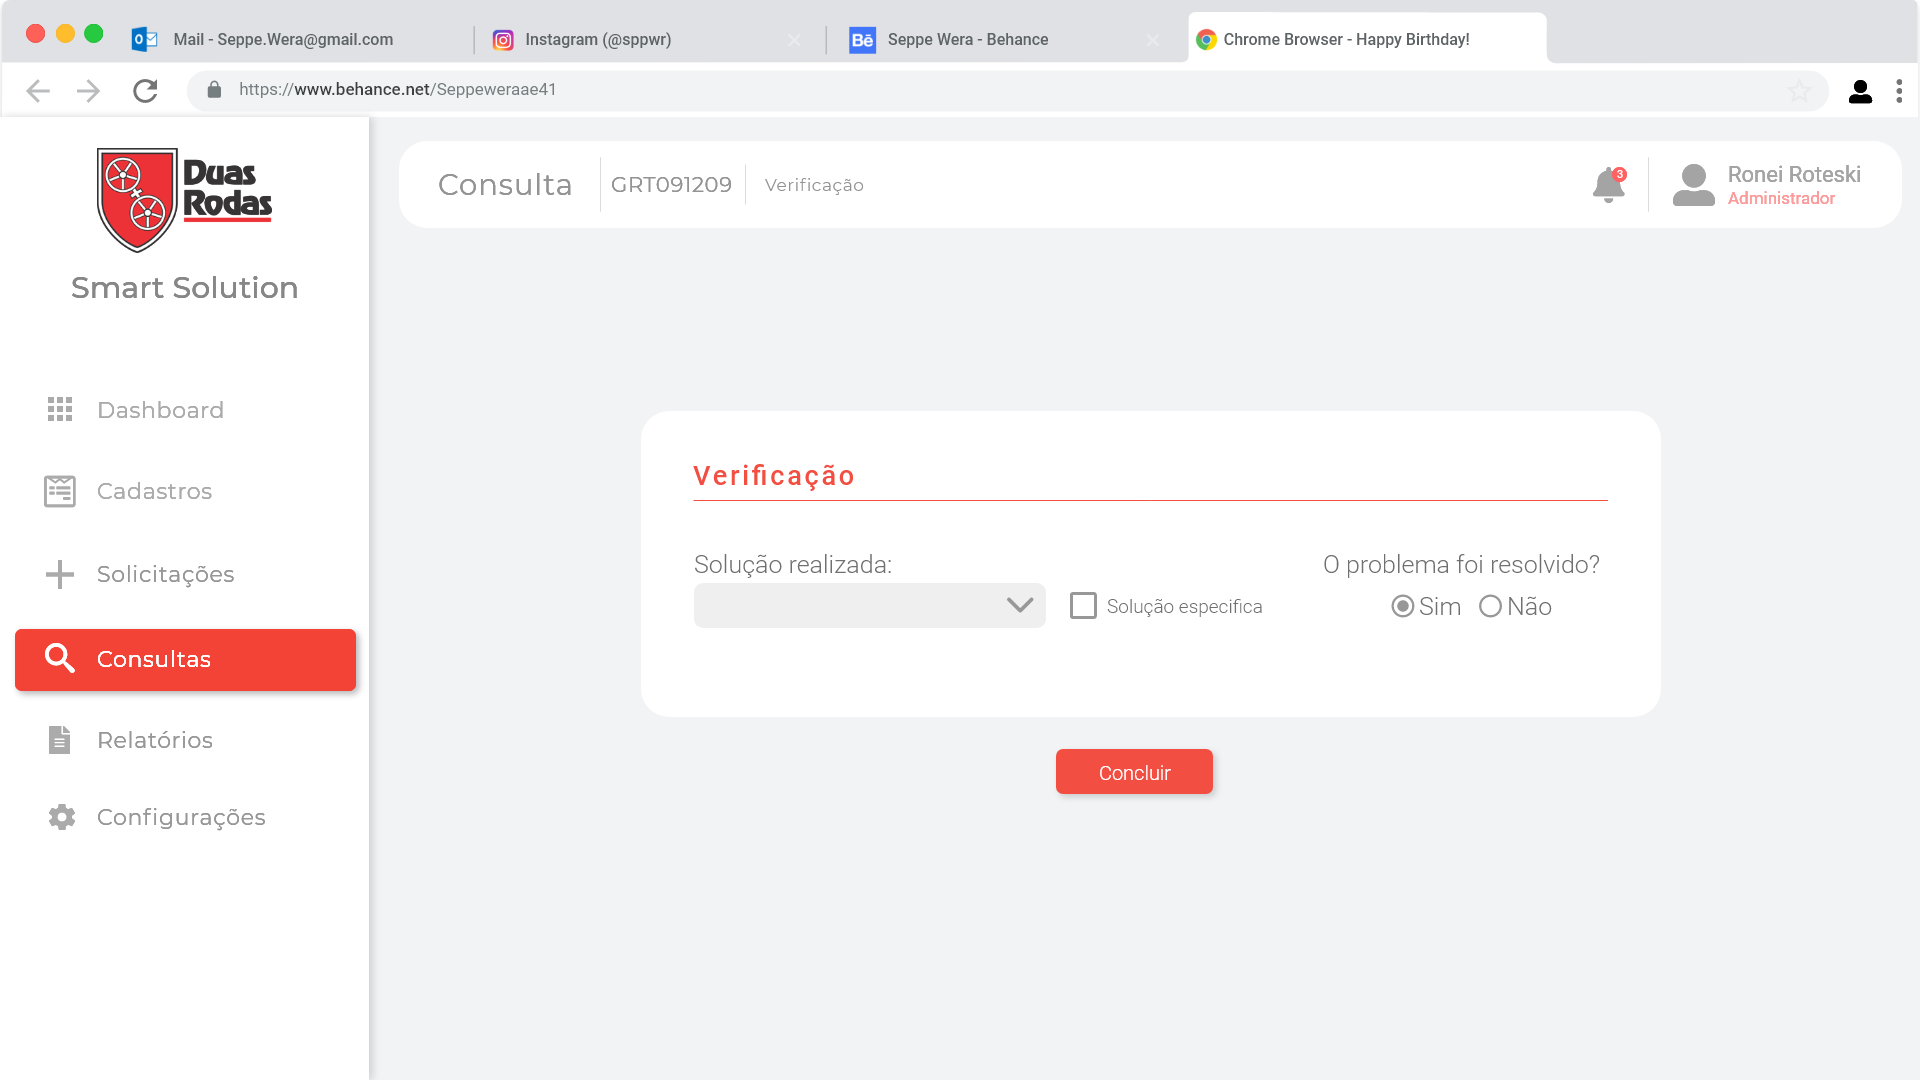
\includegraphics[scale=.32,angle=90]{Figuras/Verificacao_web}}\qquad
	}
	
\end{figure}
\newpage

Tela para apontar horas trabalhadas.
\begin{figure}[htb]
	\centering
	\mbox{%
		\subfigure[Tela de Apontamento]{\label{APONTAMENTO_web}%
			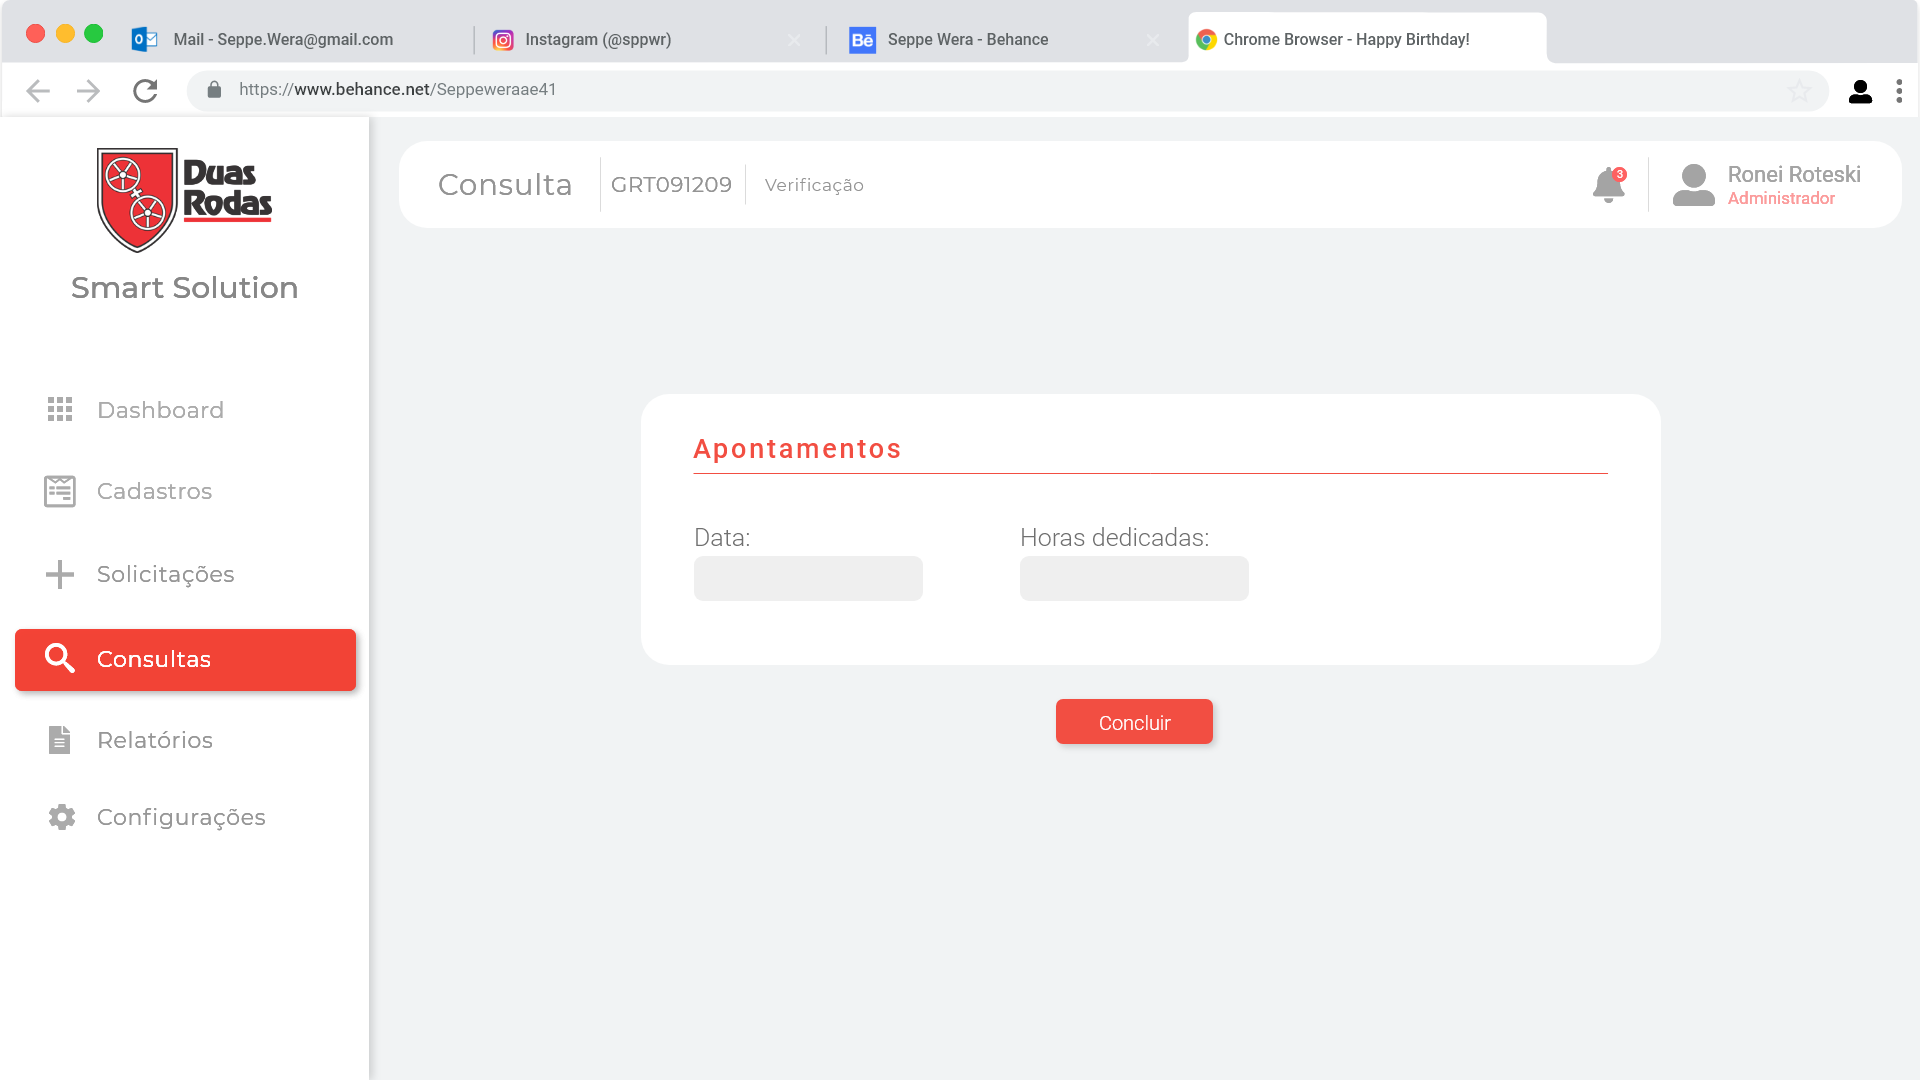
\includegraphics[scale=.32,angle=90]{Figuras/APONTAMENTO_web}}\qquad
	}
	
\end{figure}
\newpage
Tela para verificar se possui todas as assinaturas.
\begin{figure}[htb]
	\centering
	\mbox{%
		\subfigure[Tela de Assinatura]{\label{Assinatura_web}%
			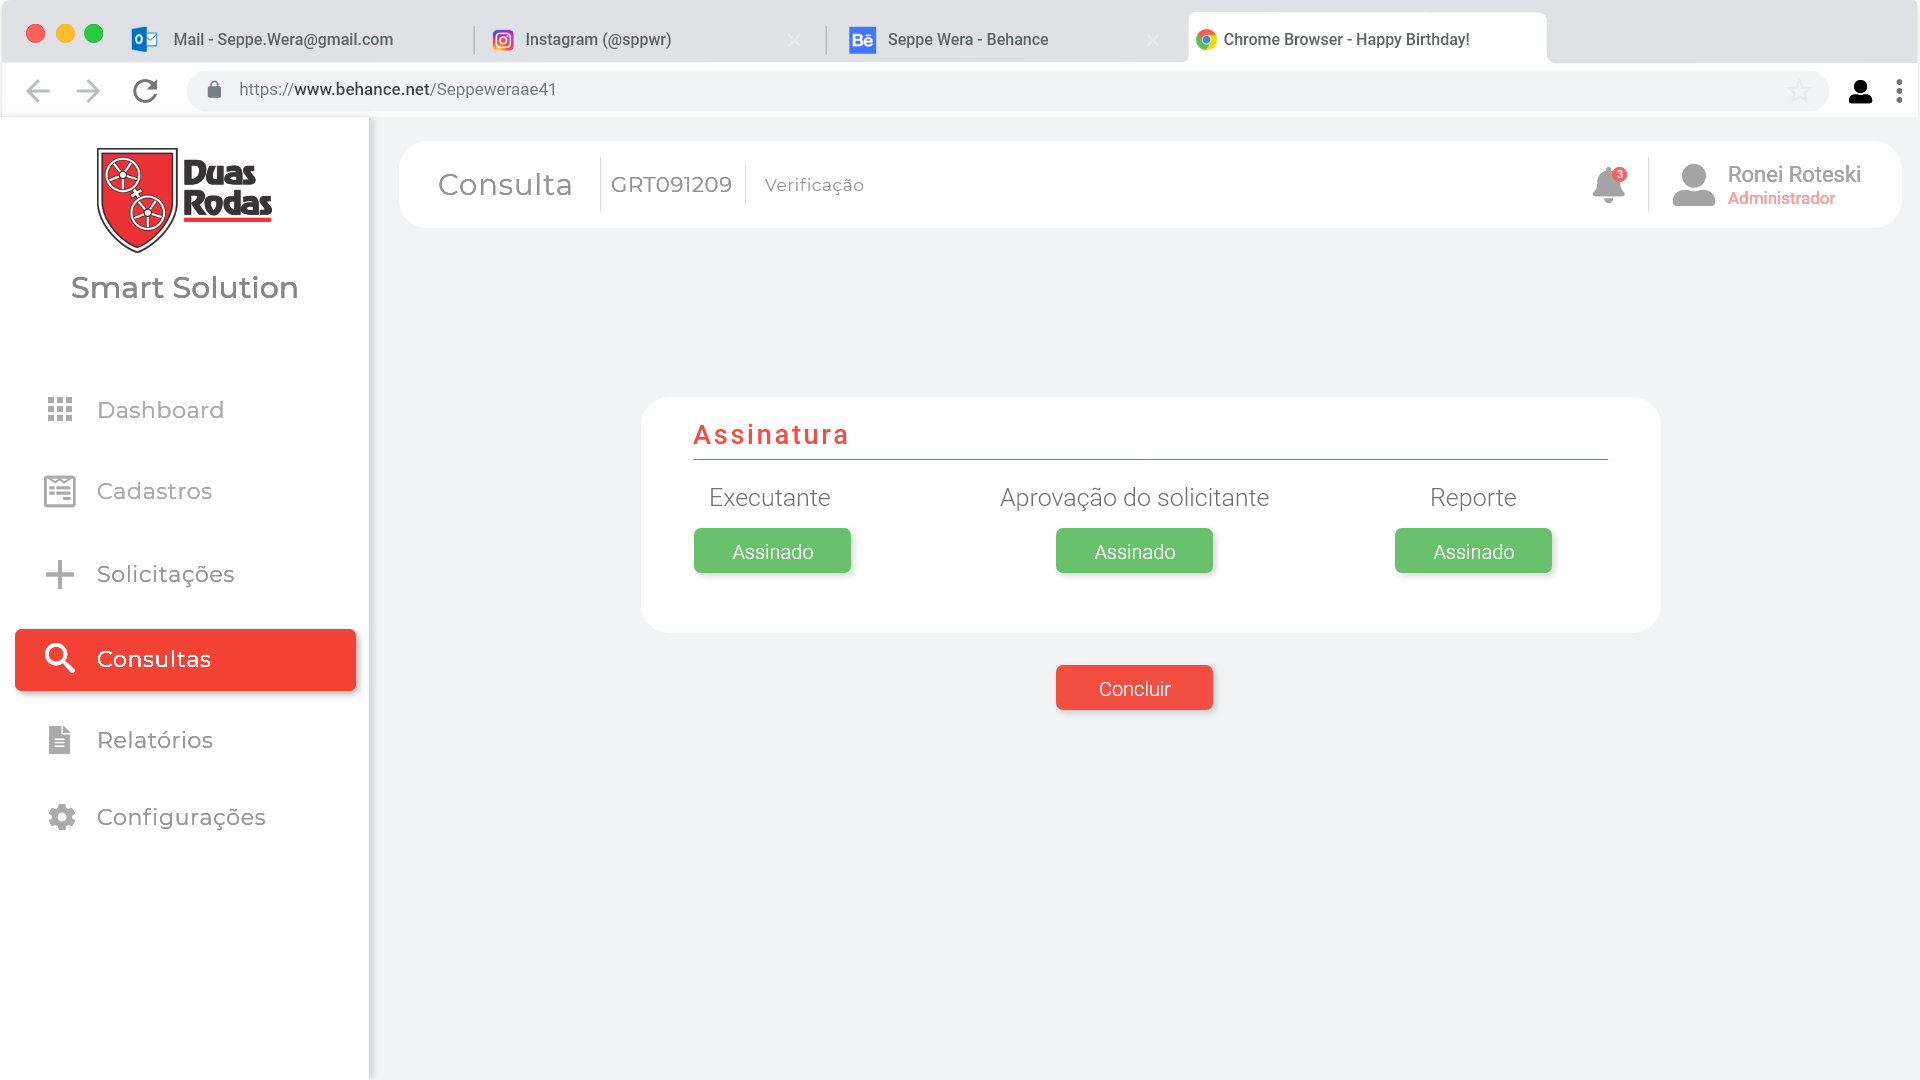
\includegraphics[scale=.32,angle=90]{Figuras/Assinatura_web}}\qquad
	}
	
\end{figure}
\newpage

Telas de relatórios parte 1.
\begin{figure}[htb]
	\centering
	\mbox{%
		\subfigure[Tela de relatórios 1]{\label{Relatorios}%
			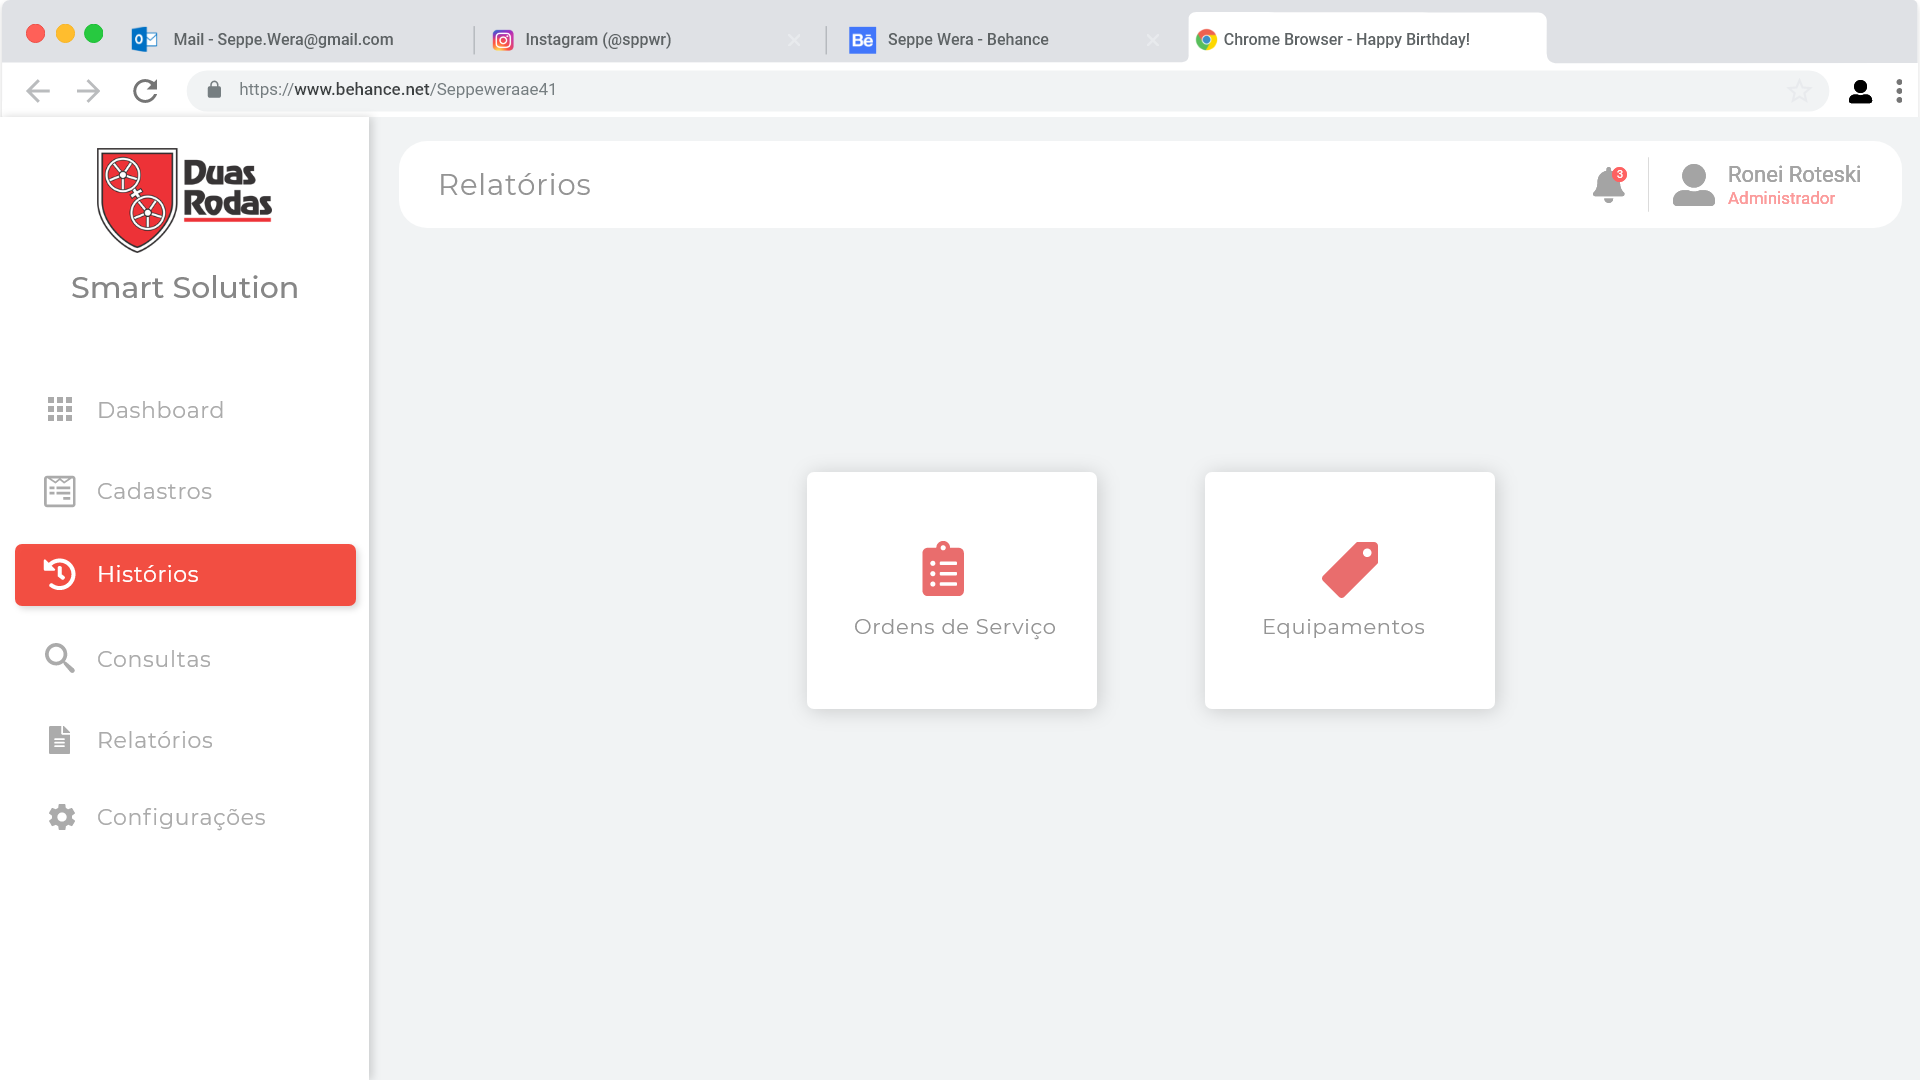
\includegraphics[scale=.32,angle=90]{Figuras/Relatorios}}\qquad
	}
	
\end{figure}
\newpage
Telas de relatórios parte 2.
\begin{figure}[htb]
	\centering
	\mbox{%
		\subfigure[Tela de relatórios 2]{\label{Relatorios_1}%
			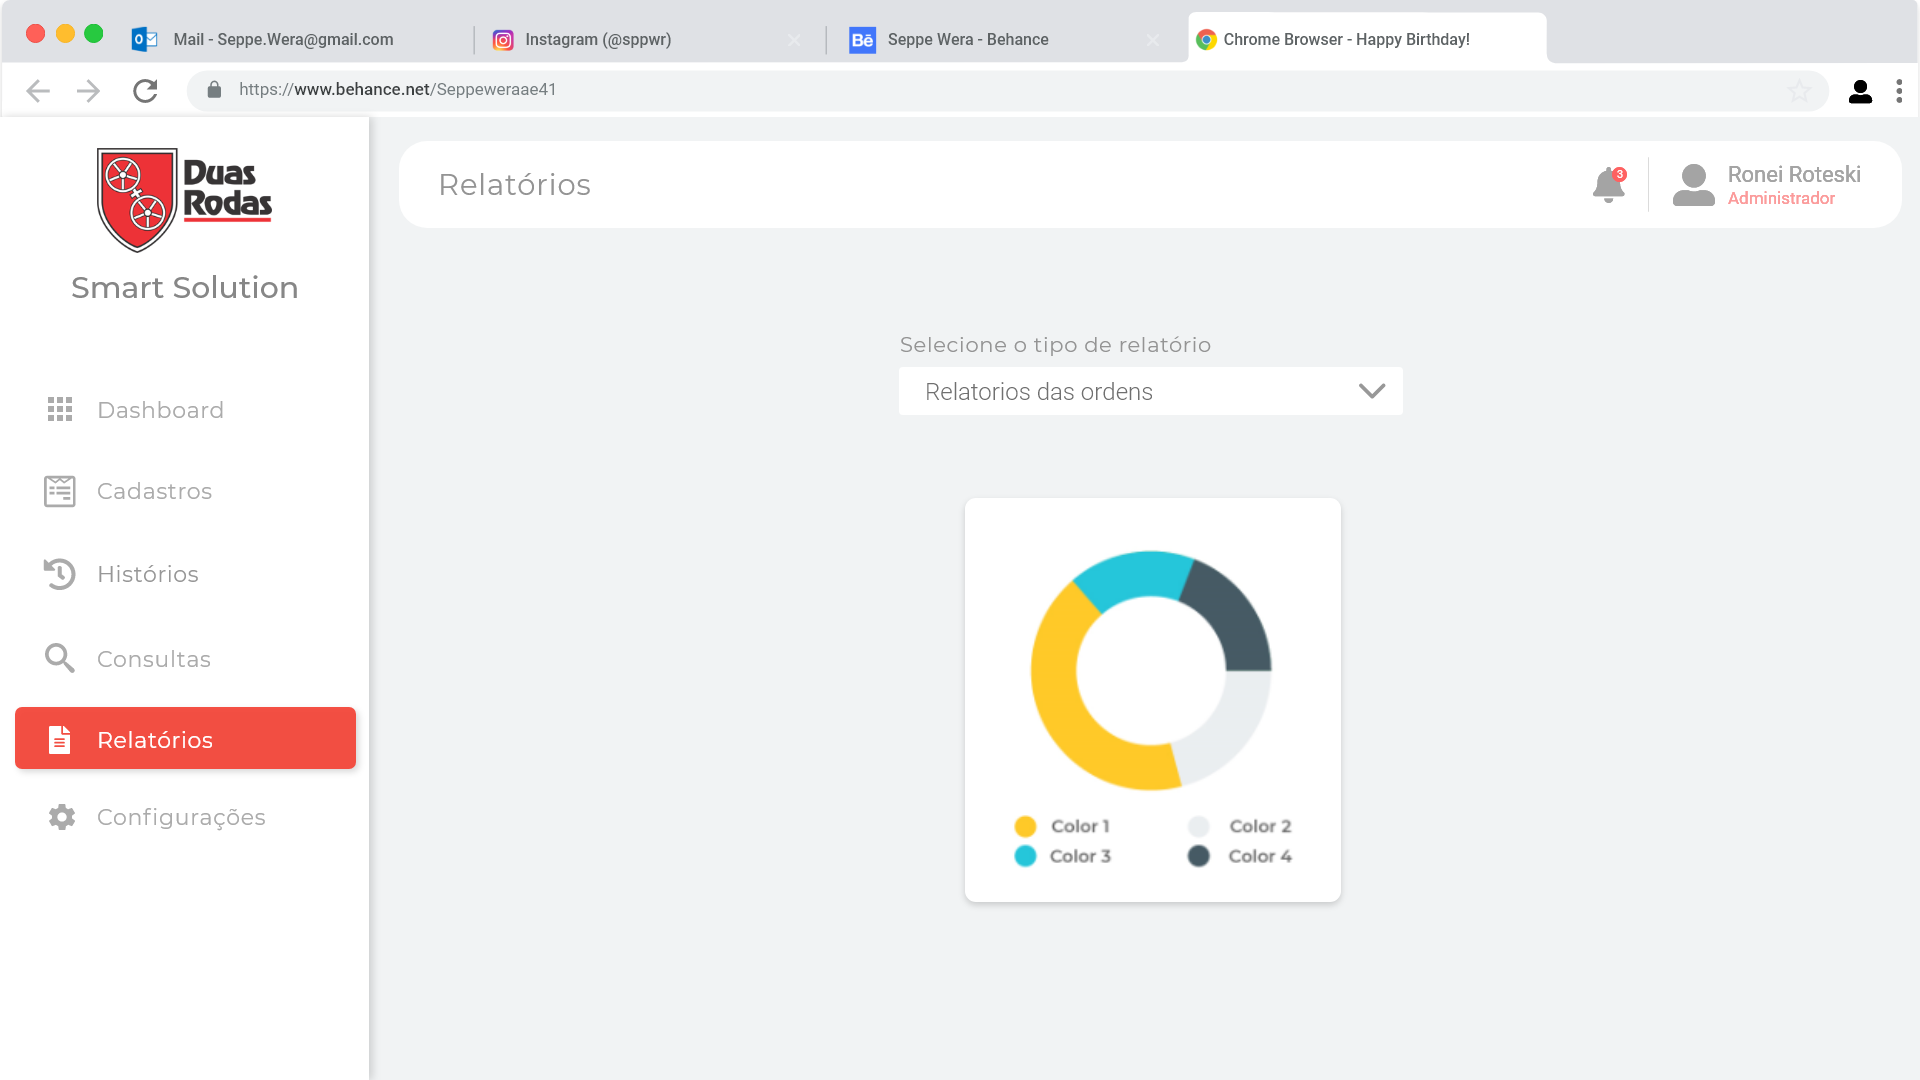
\includegraphics[scale=.32,angle=90]{Figuras/Relatorios_1}}\qquad
	}
	
\end{figure}
\newpage
Telas de relatórios mensais parte 1.
\begin{figure}[htb]
	\centering
	\mbox{%
		\subfigure[Tela de relatórios mensais 1]{\label{Relatorios_mensais}%
			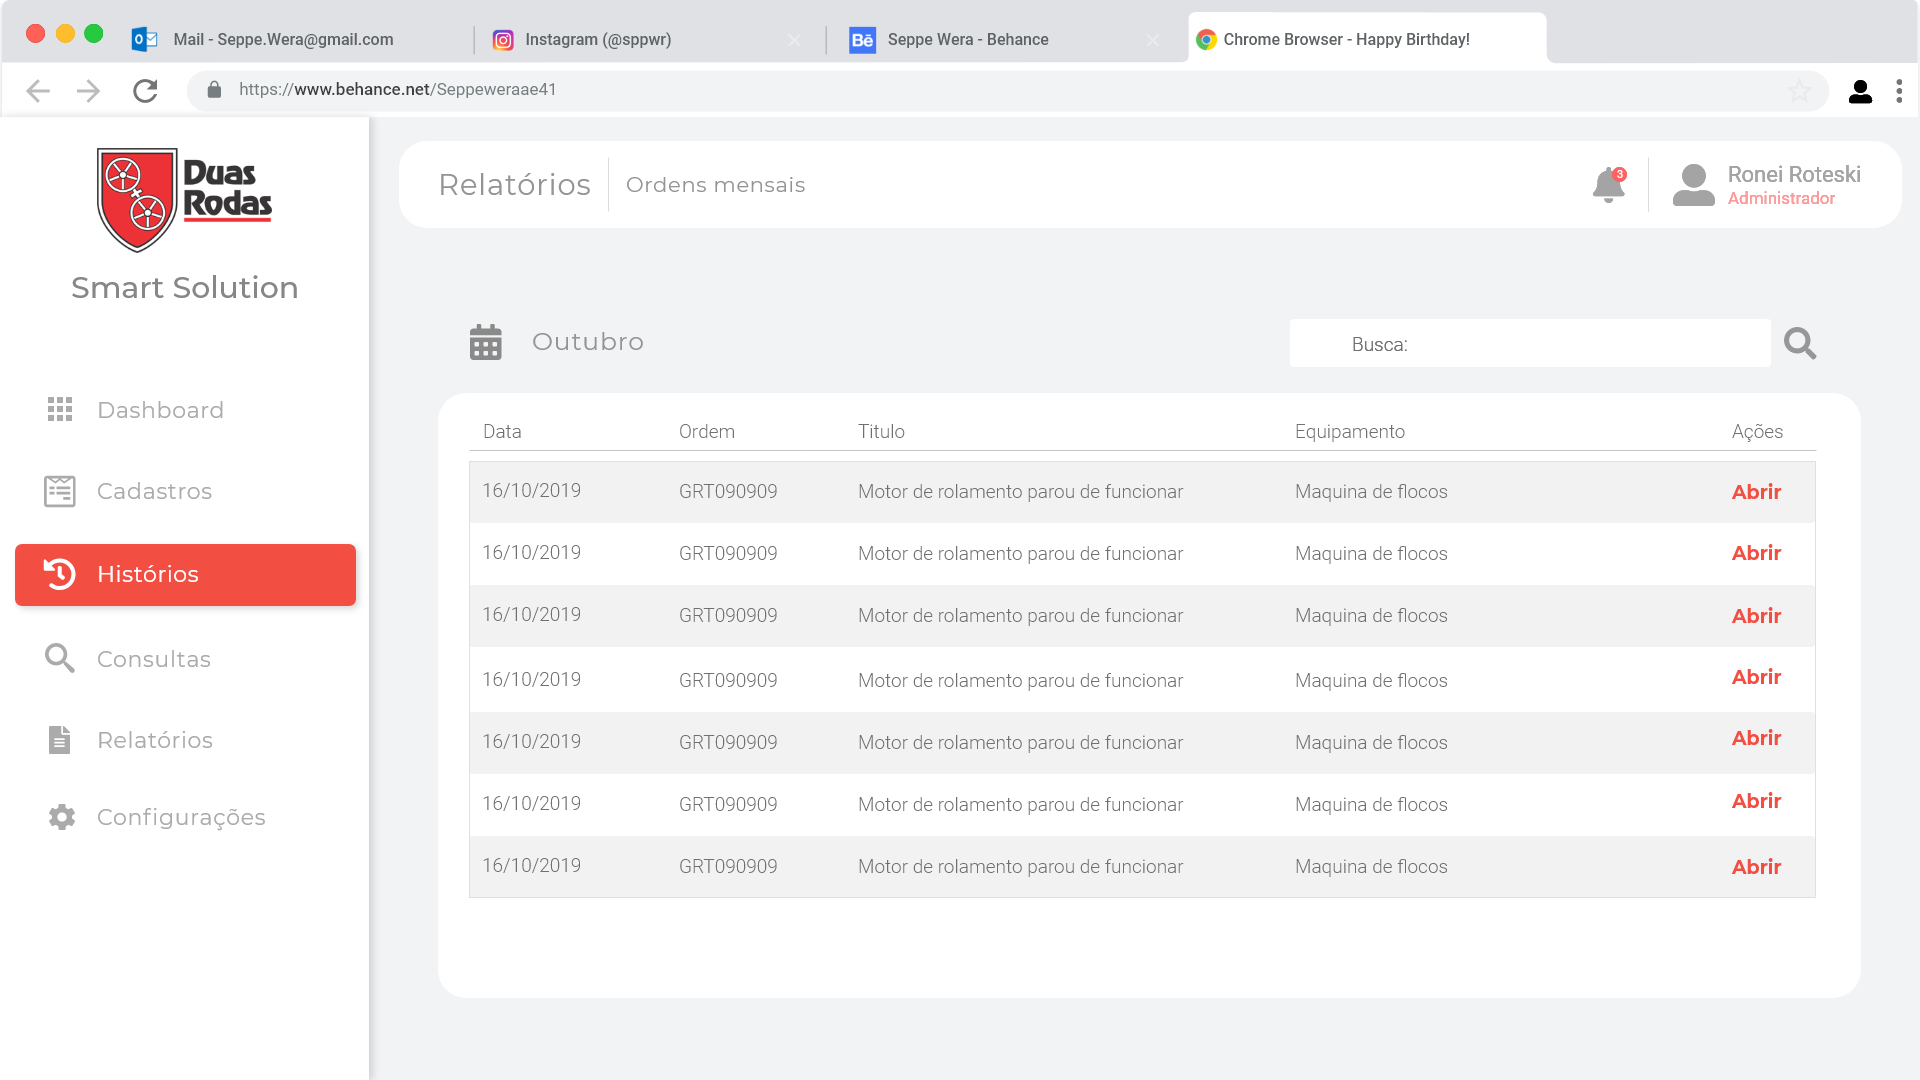
\includegraphics[scale=.32,angle=90]{Figuras/Relatorios_mensais}}\qquad
	}
	
\end{figure}
\newpage
Telas de relatórios mensais parte 2.
\begin{figure}[htb]
	\centering
	\mbox{%
		\subfigure[Tela de relatórios mensais 2]{\label{Relatorios_mensais _1}%
			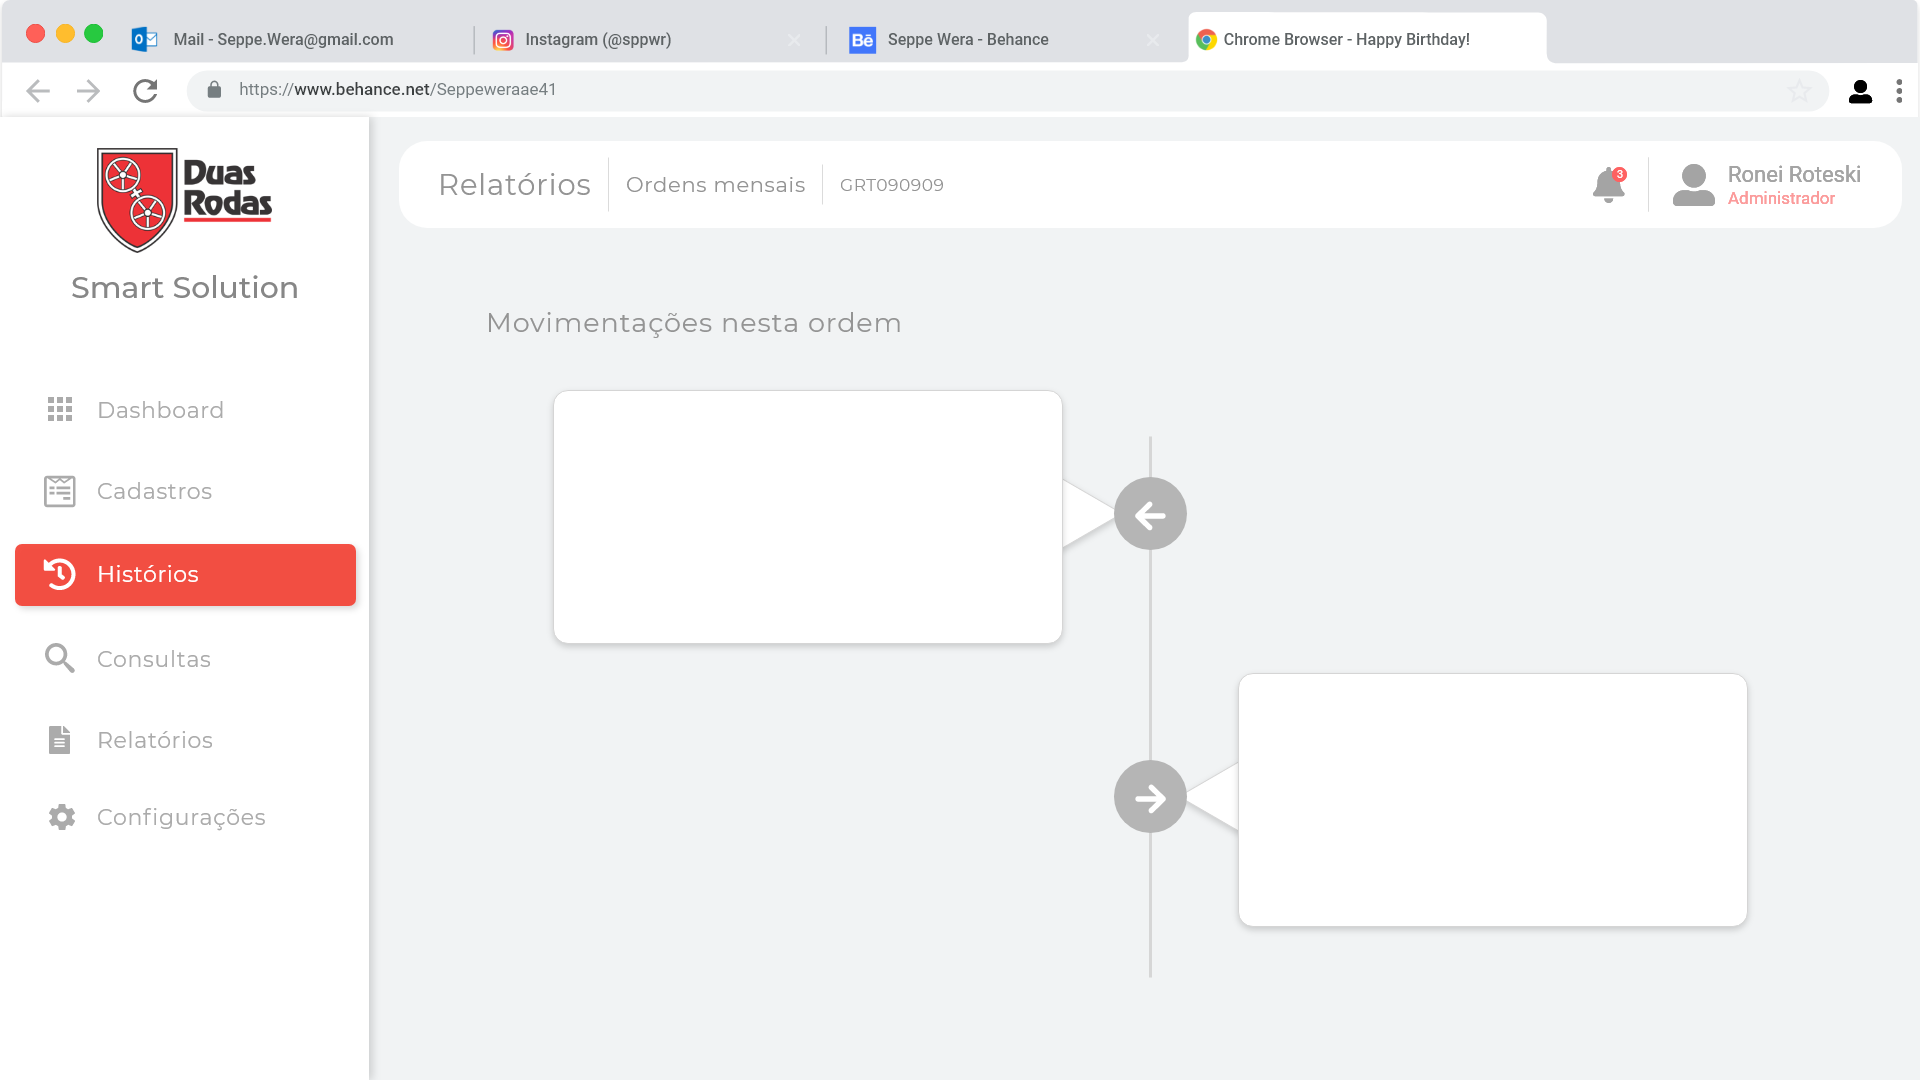
\includegraphics[scale=.32,angle=90]{Figuras/Relatorios_mensais _1}}\qquad
	}
	
\end{figure}
\newpage
Telas de relatórios mensais parte 3.
\begin{figure}[htb]
	\centering
	\mbox{%
		\subfigure[Tela de relatórios mensais 3]{\label{Relatorios_mensais _2}%
			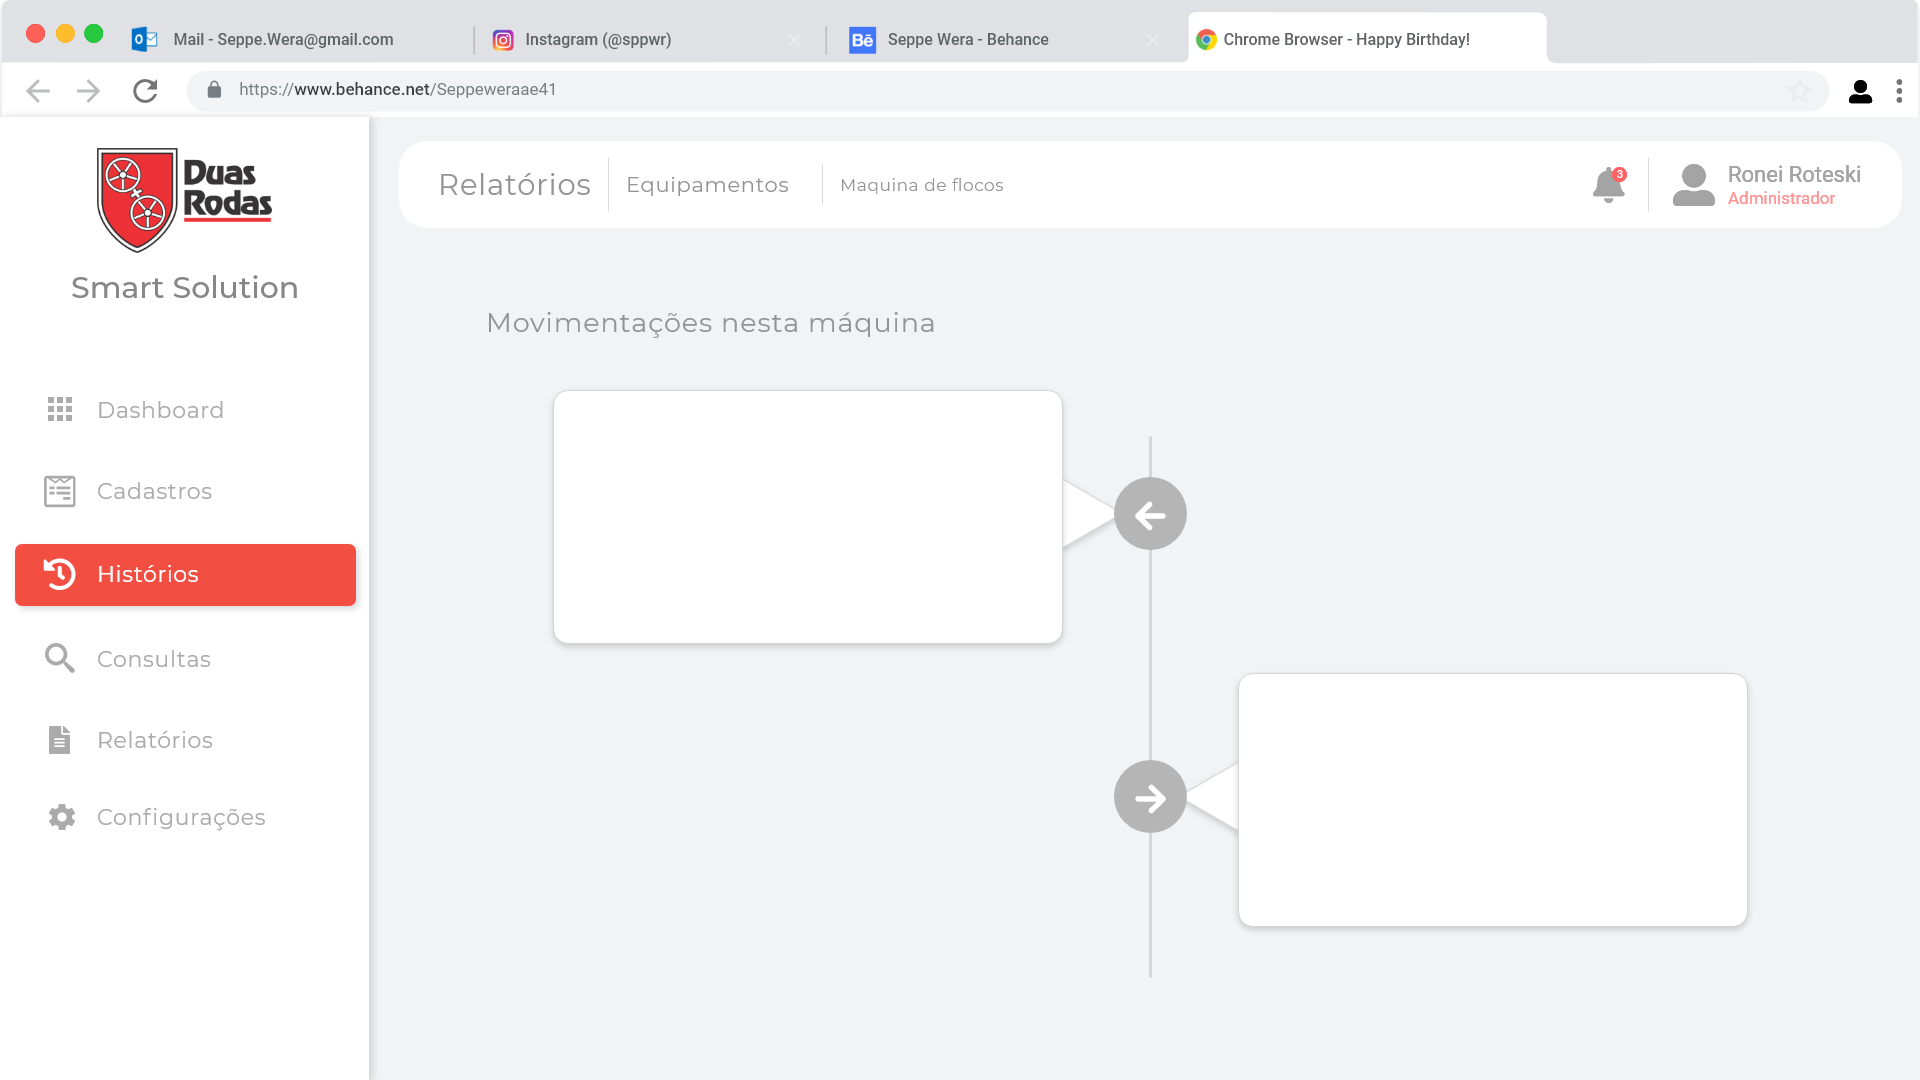
\includegraphics[scale=.32,angle=90]{Figuras/Relatorios_mensais _2}}\qquad
	}
	
\end{figure}
\newpage
Telas de relatórios de equipamentos.
\begin{figure}[htb]
	\centering
	\mbox{%
		\subfigure[Tela de relatórios equipamentos]{\label{Relatorios_por_equipamento}%
			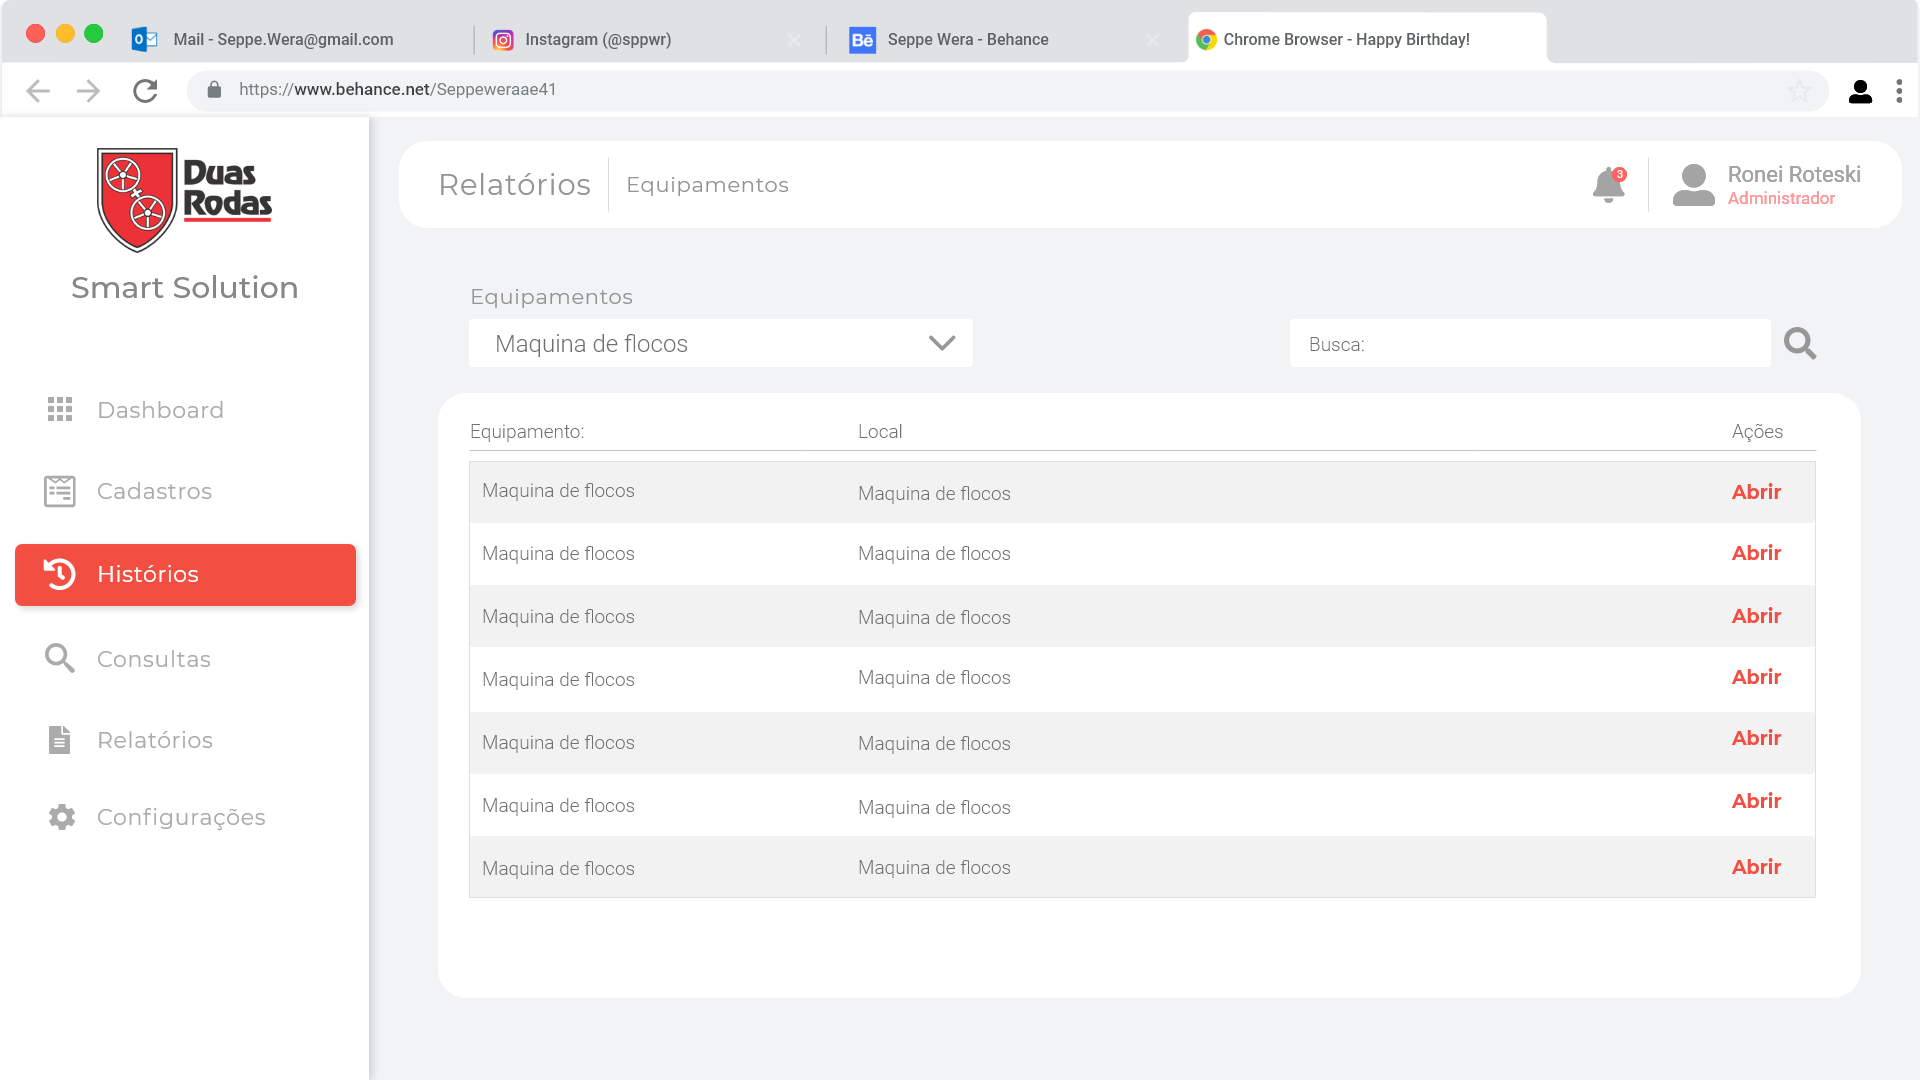
\includegraphics[scale=.32,angle=90]{Figuras/Relatorios_por_equipamento}}\qquad
	}
	
\end{figure}

\newpage
Tela assinatura apos a verificação dos procedimentos realizados realizados pelo funcionário, que contem também a opção assinatura do solicitante da OS.

\begin{figure}[htb]
	\centering
	\mbox{%
		\subfigure[Tela de assinatura]{\label{verificacao_13_1}%
			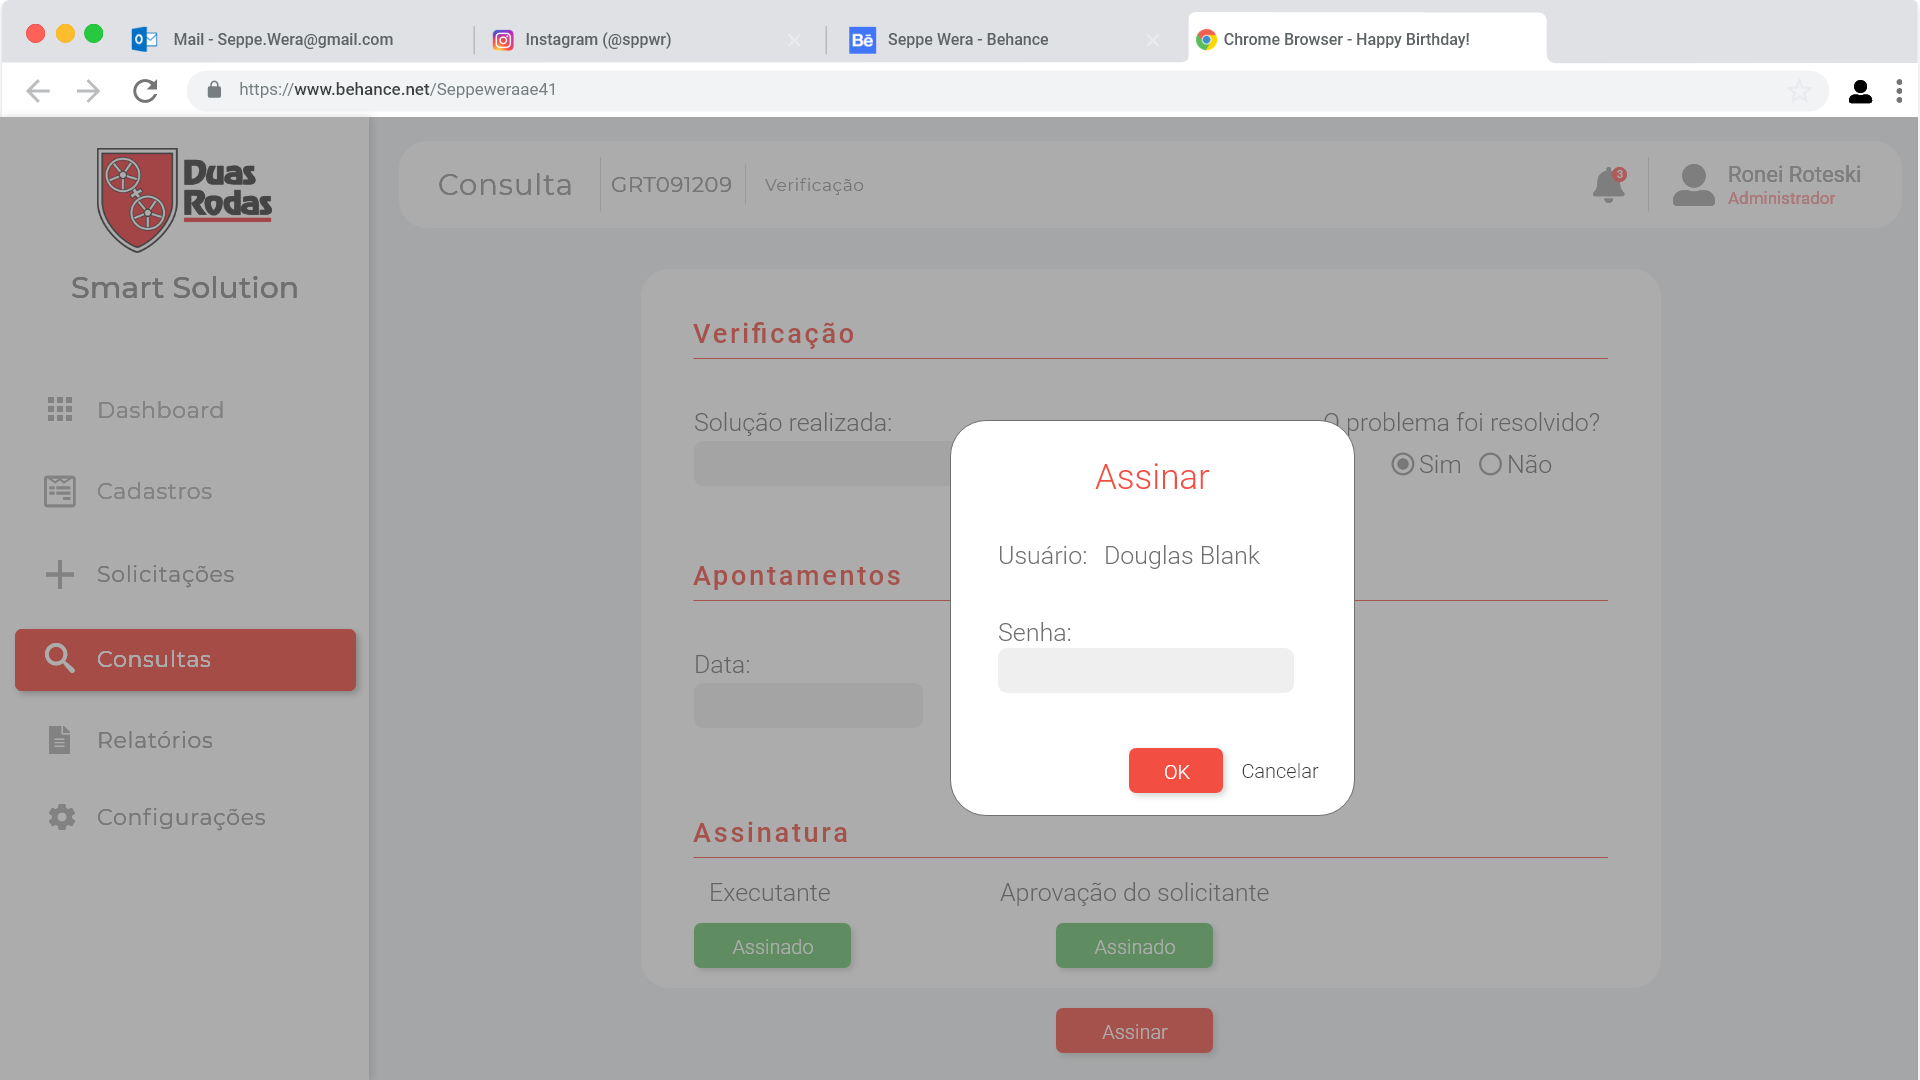
\includegraphics[scale=.32,angle=90]{Figuras/verificacao_13_1}}\qquad
	}
	
\end{figure}
\newpage
Tela de Checklist dos Equipamento de proteção individual do funcionário.

\begin{figure}[htb]
	\centering
	\mbox{%
		\subfigure[Tela de Checklist EPI]{\label{CHECKLIST_14}%
			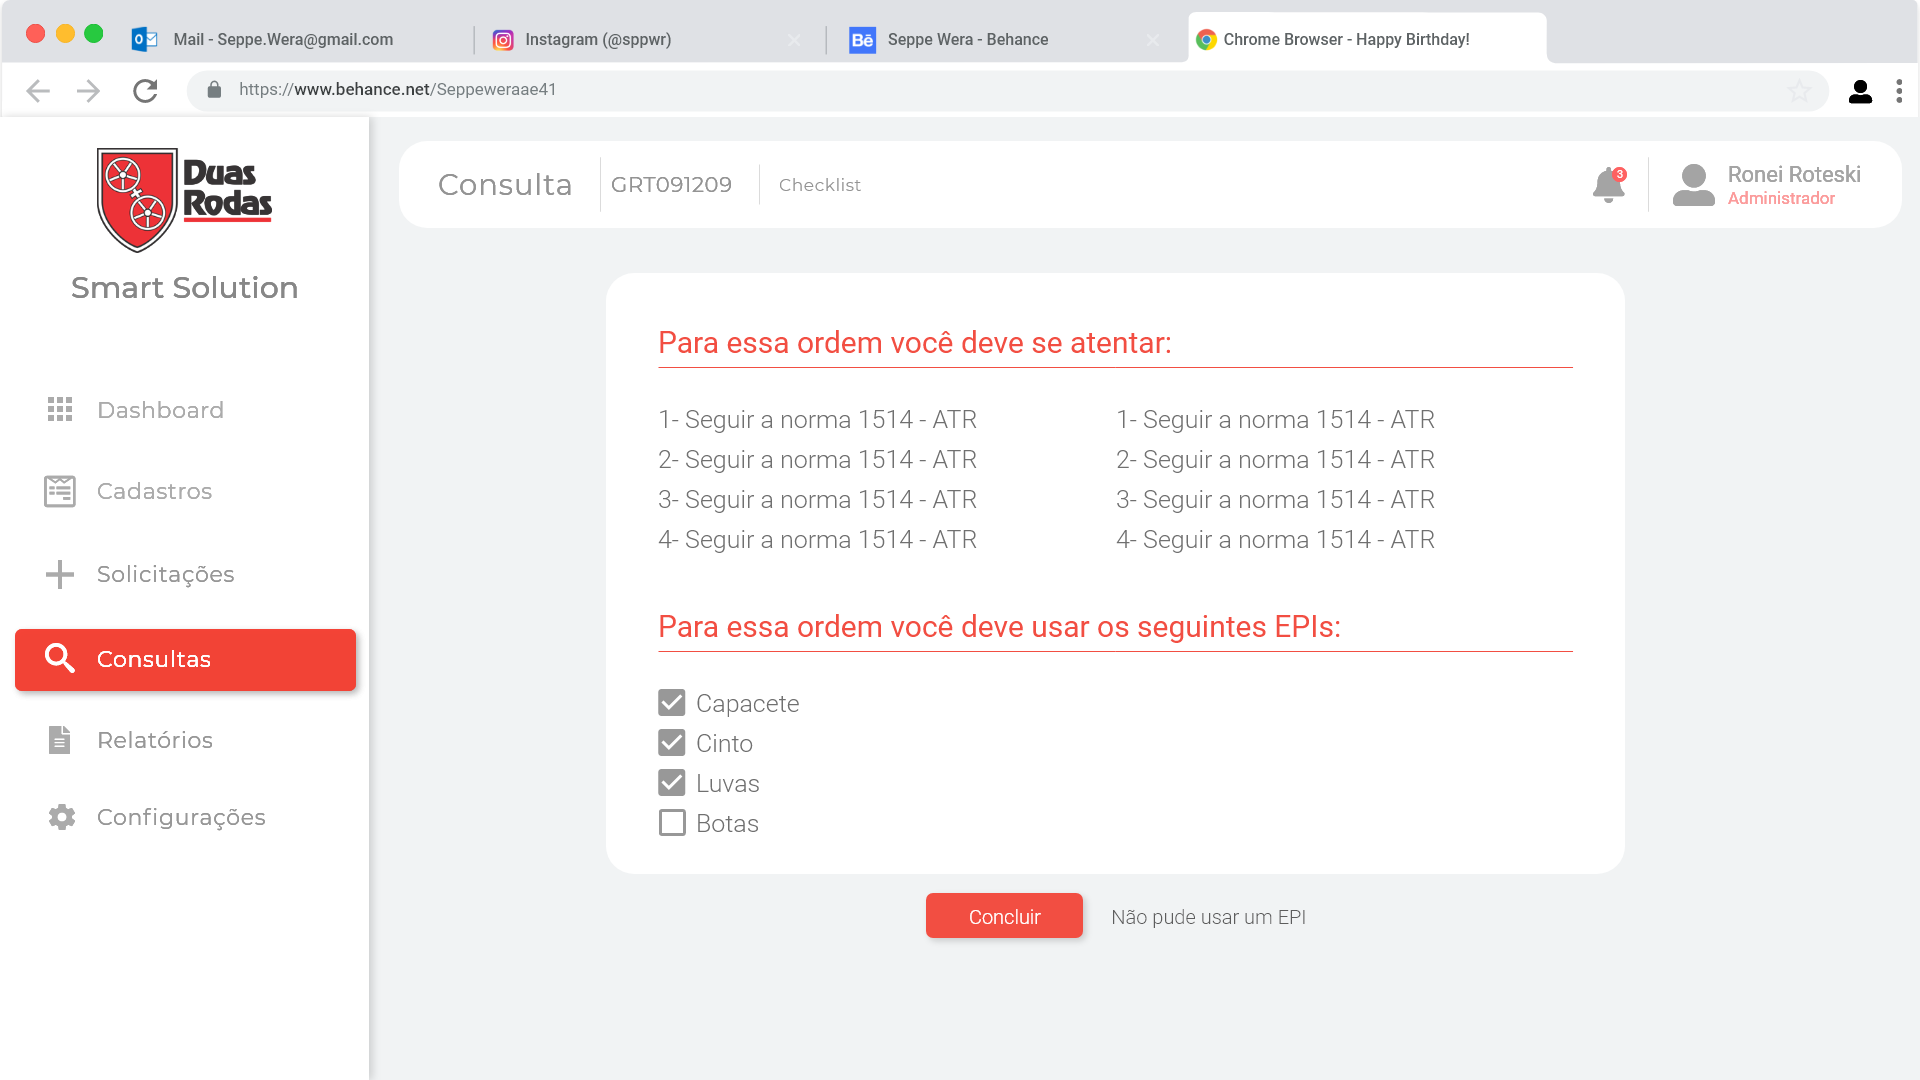
\includegraphics[scale=.32,angle=90]{Figuras/CHECKLIST_14}}\qquad
	}
	
\end{figure}
\newpage
Tela para se justificação do motivo por não utilizar algum EPI especifico.

\begin{figure}[htb]
	\centering
	\mbox{%
		\subfigure[Tela justificação não uso EPI]{\label{CHECKLIST_14_1}%
			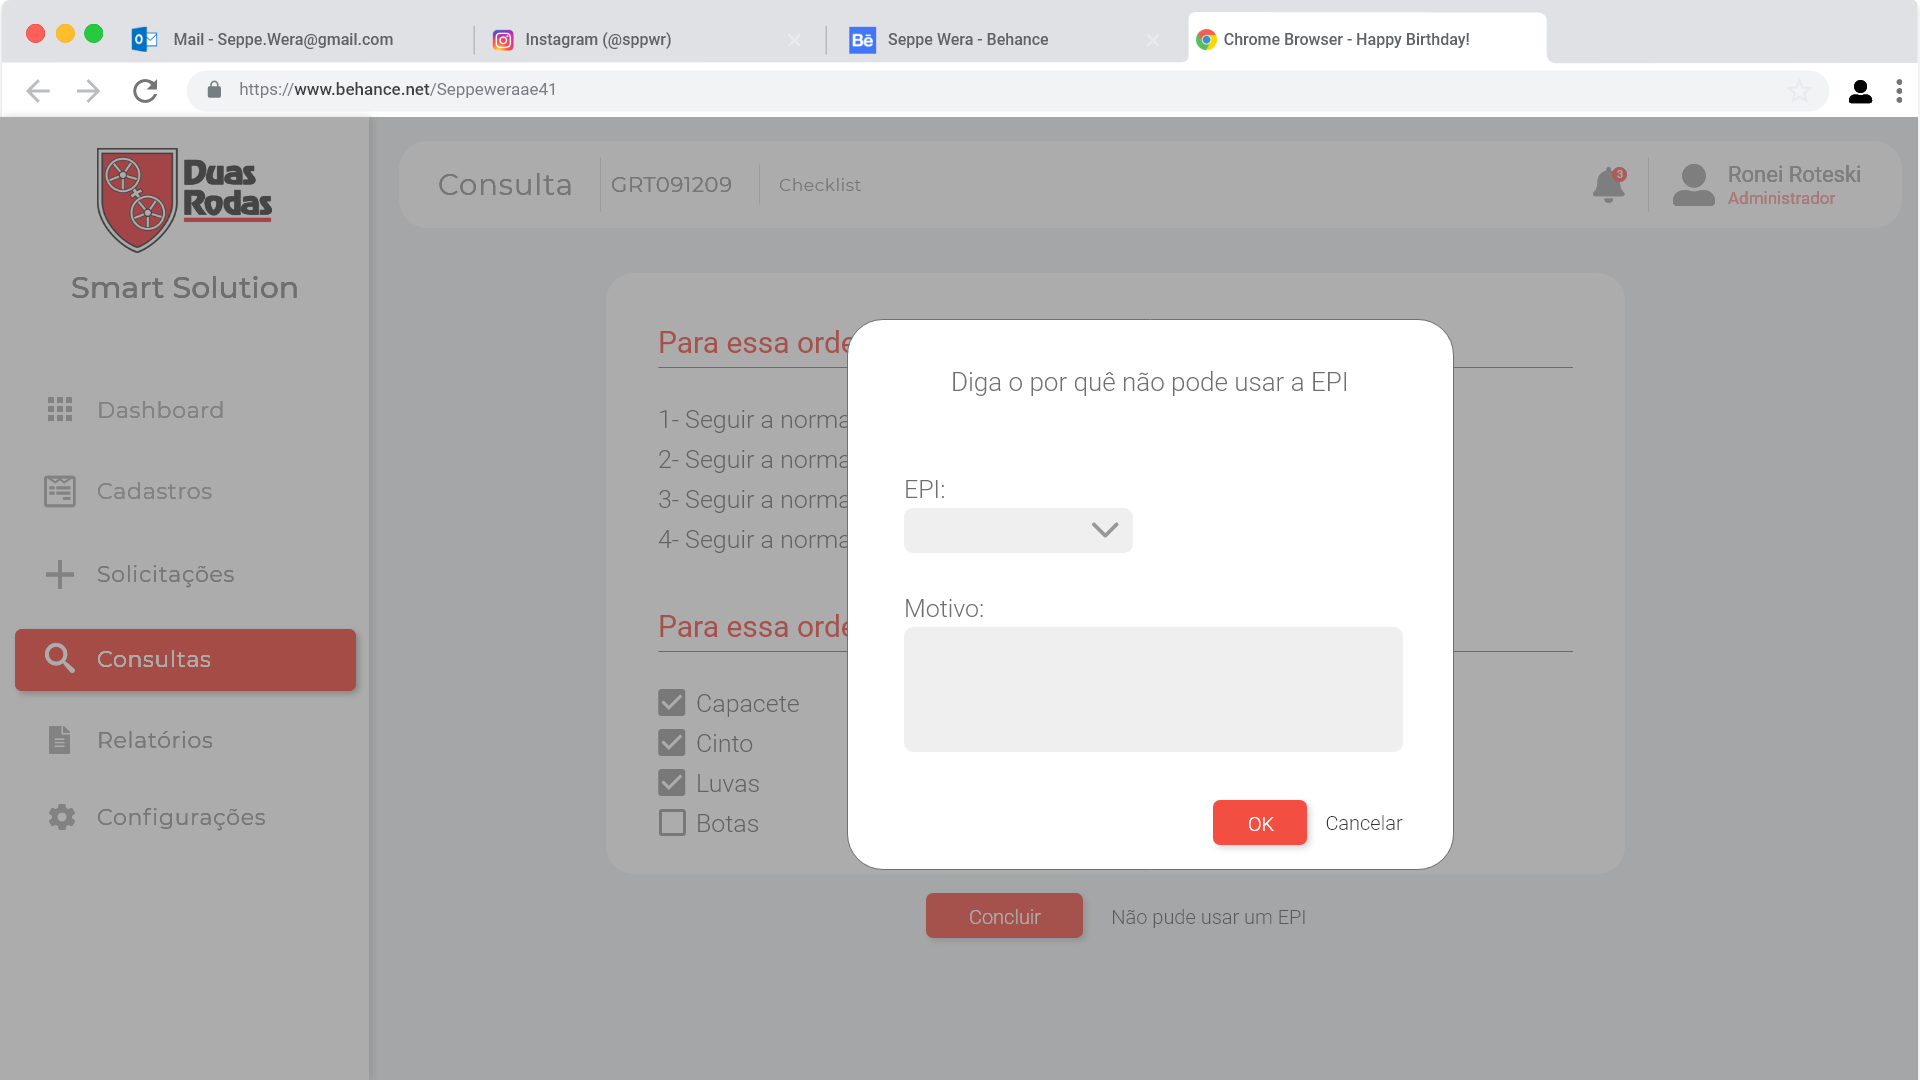
\includegraphics[scale=.32,angle=90]{Figuras/CHECKLIST_14_1}}\qquad
	}
	
\end{figure}
\newpage
Tela de assinatura dos responsáveis pela manutenção, solicitante e do administrador.

\begin{figure}[htb]
	\centering
	\mbox{%
		\subfigure[Tela com assinatura dos  responsáveis]{\label{ASSINATURA_15}%
			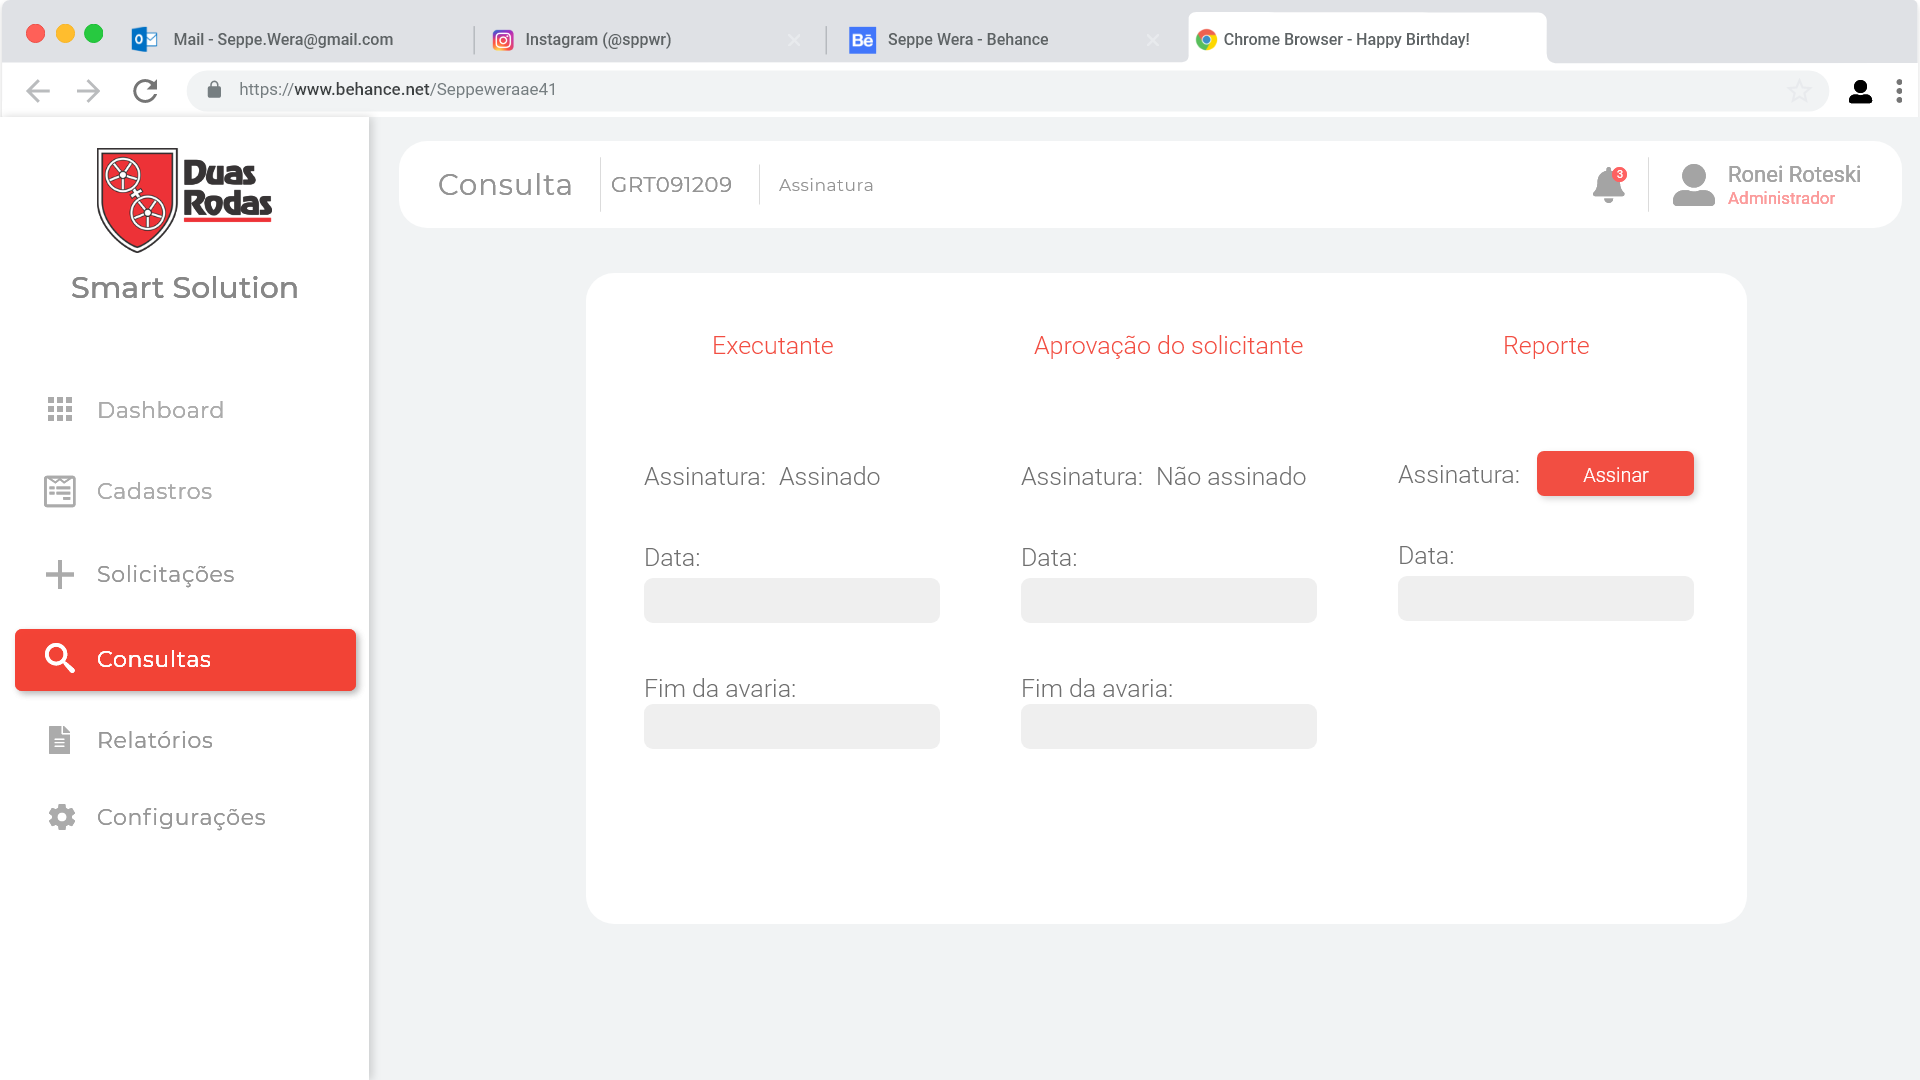
\includegraphics[scale=.32,angle=90]{Figuras/ASSINATURA_15}}\qquad
	}
	
\end{figure}
\newpage
Tela para cadastrar usuários novos no sistema.

\begin{figure}[htb]
	\centering
	\mbox{%
		\subfigure[Tela para cadastrar usuário]{\label{CADASTRAR_USUARIO_16}%
			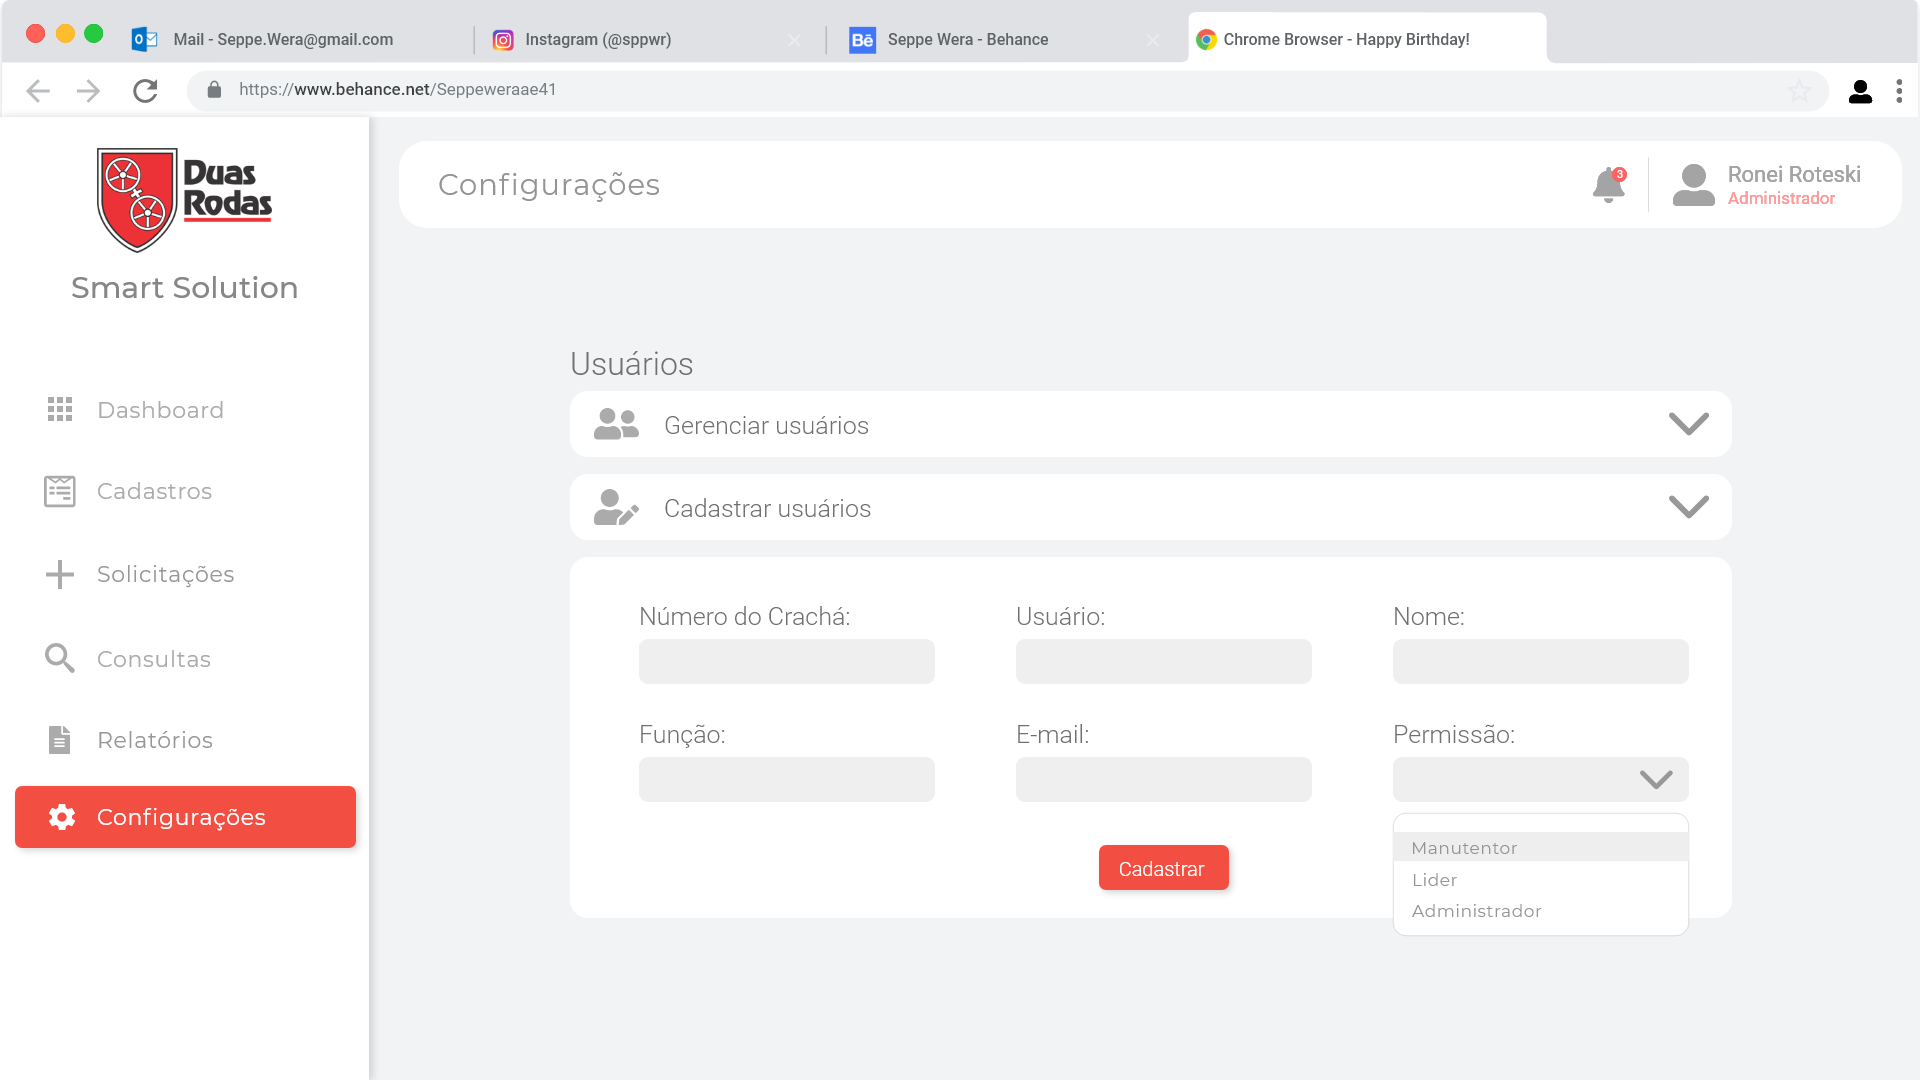
\includegraphics[scale=.32,angle=90]{Figuras/CADASTRAR_USUARIO_16}}\qquad
	}
	
\end{figure}


\newpage